\documentclass[12pt]{article}
%\usepackage[utf8]{inputenc}
\usepackage{indentfirst}
\usepackage{float}
\usepackage{array}
\usepackage{url}
\urlstyle{tt}
\usepackage{enumitem, amsmath, amssymb, amsfonts, latexsym, mathrsfs}
\usepackage{graphicx}
\usepackage{subfig}
\usepackage{multicol}
\usepackage{booktabs}
\usepackage{ragged2e}
\usepackage{svg}
\usepackage{xcolor}

\usepackage{listings}
\usepackage{atkinson} %% Option 'sfdefault' if the base
%% font of the document is to be sans serif.
\usepackage[T1]{fontenc}
\setmainfont{Atkinson Hyperlegible}
\renewcommand{\familydefault}{\sfdefault}

\usepackage[spanish]{babel}
\usepackage[utf8]{inputenc}
\usepackage[backend=biber]{biblatex}
\bibliography{referencias}
\usepackage{csquotes}
%New colors defined below
\usepackage{}
\definecolor{codegreen}{rgb}{0,0.6,0}
\definecolor{codegray}{rgb}{0.5,0.5,0.5}
\definecolor{codepurple}{rgb}{0.58,0,0.82}
\definecolor{backcolour}{rgb}{0.95,0.95,0.92}
\lstdefinestyle{mystyle}{
  backgroundcolor=\color{backcolour},   commentstyle=\color{codegreen},
  keywordstyle=\color{magenta},
  numberstyle=\tiny\color{codegray},
  stringstyle=\color{codepurple},
  basicstyle=\ttfamily\footnotesize,
  breakatwhitespace=false,         
  breaklines=true,                 
  captionpos=b,                    
  keepspaces=true,                 
  numbers=left,                    
  numbersep=5pt,                  
  showspaces=false,                
  showstringspaces=false,
  showtabs=false,                  
  tabsize=2
}
%"mystyle" code listing set
\lstset{style=mystyle}
%\lstset{basicstyle=\ttfamily\footnotesize,breaklines=true}

\usepackage{notoccite}

\usepackage{multicol}
\setlength{\columnseprule}{1pt}
\def\columnseprulecolor{\color{black}}





\date{}
% Comand para keywords
\providecommand{\keywords}[1]
{
  \small	
  \textbf{\textit{Keywords---}} #1
}

% Tipografía
%\usepackage{helvet}
%\renewcommand{\familydefault}{\sfdefault}
%\usepackage[sfdefault]{Chivo}
%\usepackage{comment}


\urlstyle{same}
% \tolerance=9999
% \emergencystretch=10pt
\hyphenpenalty=10000
\sloppy
% \exhyphenpenalty=100

\renewcommand{\figurename}{\textbf{Figura.}}
\renewcommand\spanishtablename{Tabla.}

% Interlineado
\usepackage{setspace}
\spacing{1.15}

% Márgenes
\usepackage[a4paper]{geometry}
\geometry{top=2.5cm, bottom=2.5cm, left=2cm, right=2cm}

% Número de página
\usepackage{fancyhdr}
\pagestyle{fancy}
\rhead[]{}
\lhead[]{}
\renewcommand{\headrulewidth}{0pt}
\rfoot[]{\thepage}
\cfoot[]{}

\usepackage[breaklinks]{hyperref}
% Setup de hiperenlaces
\hypersetup{
    colorlinks=true,
    linkcolor=blue,
    filecolor=magenta,      
    urlcolor=cyan,
    pdftitle={Arquitectura de las consolas de videojuegos},
    pdfpagemode=FullScreen,
    citecolor = green
    }
\usepackage[norule]{footmisc}

%_____________________________________________________________________________
%_____________________________________________________________________________
%_____________________________________________________________________________
%_____________________________________________________________________________
\hbadness=50000
\usepackage{microtype}
\begin{document}
\nocite{atkinson}
\nocite{circuitverse}
\nocite{chatgpt}
\nocite{duke}
% PORTADA        
\begin{titlepage}
        \begin{center}
             
         
        \hrule
        \vspace{1cm}
        %{\bfseries\Large UNIVERSIDAT JAUME I \par}
        \vspace{1cm}
        {\bfseries\huge Apuntes de Consolas y Dispositivos de Videojuegos \par}
        \vspace{2cm}

        \begin{figure}[H]
            \centering
            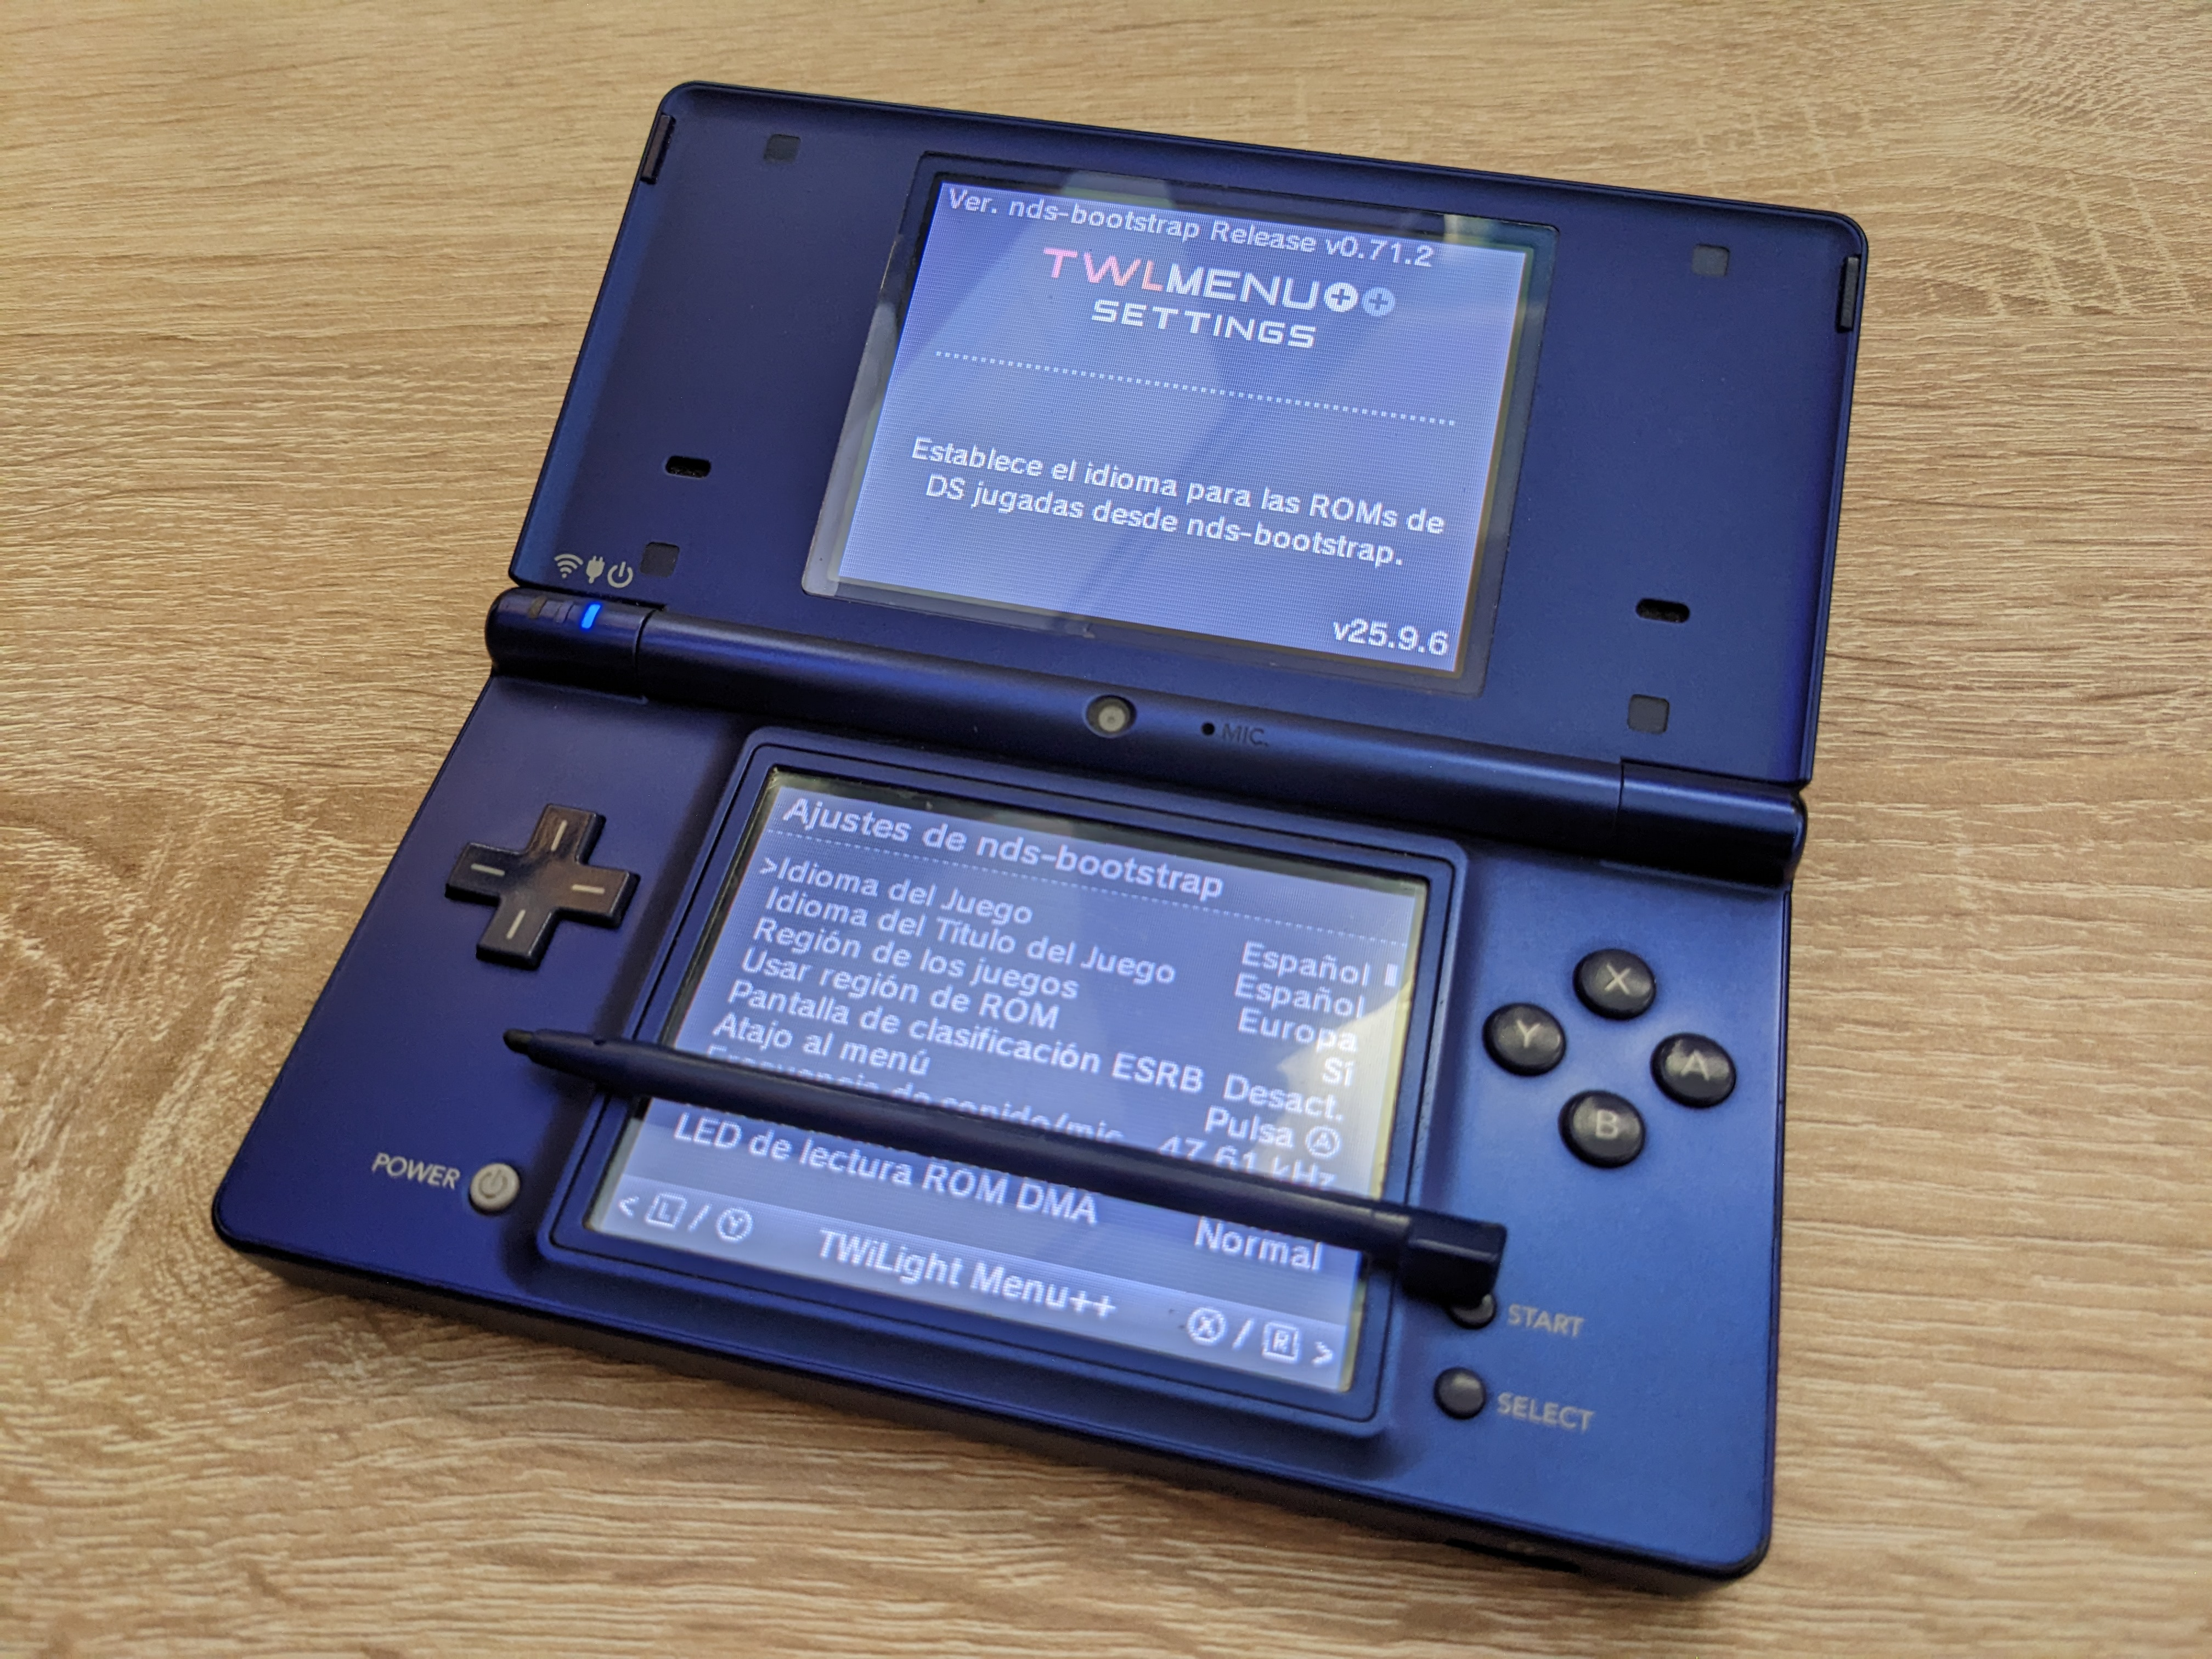
\includegraphics[width=\textwidth]{dsi.jpg}
            \caption*{\footnotesize{\textit{Nintendo DSi con Homebrew y emulador de NDS}}}
            \label{fig:dsi}
        \end{figure}
        
        {\large 
        Jesús Jiménez Montero \\
        \par}
        \vspace{1cm}
        \hrule
        \vspace{1cm}

        {\large 
        \textit{Versión 3: Puertas lógicas básicas extendidas\\
        Fecha: 09/10/2023}
        \par}
        \end{center}
\end{titlepage}

% ÍNDICE
%\renewcommand{\tableofcontents}{Indice general}
\newpage
\renewcommand{\contentsname}{Tabla de contenidos}
\setcounter{secnumdepth}{5}
\tableofcontents
\setcounter{tocdepth}{4}

\newpage
%-----------------------------------------------------------------
%-----------------------------------------------------------------
% Tabla de figuras
\newpage
\renewcommand{\listfigurename}{Lista de figuras}
\thispagestyle{empty}
\listoffigures
\newpage

\renewcommand{\listtablename}{Lista de tablas}
\listoftables
\newpage

%-----------------------------------------------------------------
%-----------------------------------------------------------------

%%%%%%%%%%%%%%%%%%%%%%%%%%%%%%%%%%%%%%%%%%%%%%%%%%%%%%%%%%%%%%%%%%%%%%%%%%
%%%%%%%%%%%%%%%%%%%%%%%%%%%%%%%%%%%%%%%%%%%%%%%%%%%%%%%%%%%%%%%%%%%%%%%%%%
\section{Not16}
    \subsection{Tabla de verdad y explicación del circuito}

    Una puerta lógica Not de \textit{N}-Bits, aplica una operación booleana a cada uno de los bits en sus inputs. \cite{nisan_nand2tetris_2005}
    
        \begin{table}[H]
        \centering
        \caption{Tabla de verdad de NOT16}
        \label{tab:tab_not16}
        \resizebox{\textwidth}{!}{%
        \begin{tabular}{@{}ll@{}}
        \toprule
        \texttt{IN}               & \texttt{OUT}              \\ \midrule
        \texttt{0000000000000000} & \texttt{1111111111111111} \\
        \texttt{1111111111111111} & \texttt{0000000000000000} \\
        \texttt{0101010101010101} & \texttt{1010101010101010} \\
        \texttt{. . .}            & \texttt{. . .}            \\ \bottomrule
        \end{tabular}%
        }
        \end{table}


    \subsection{Esquema del circuito interior}
        \begin{figure}[H]
            \centering
            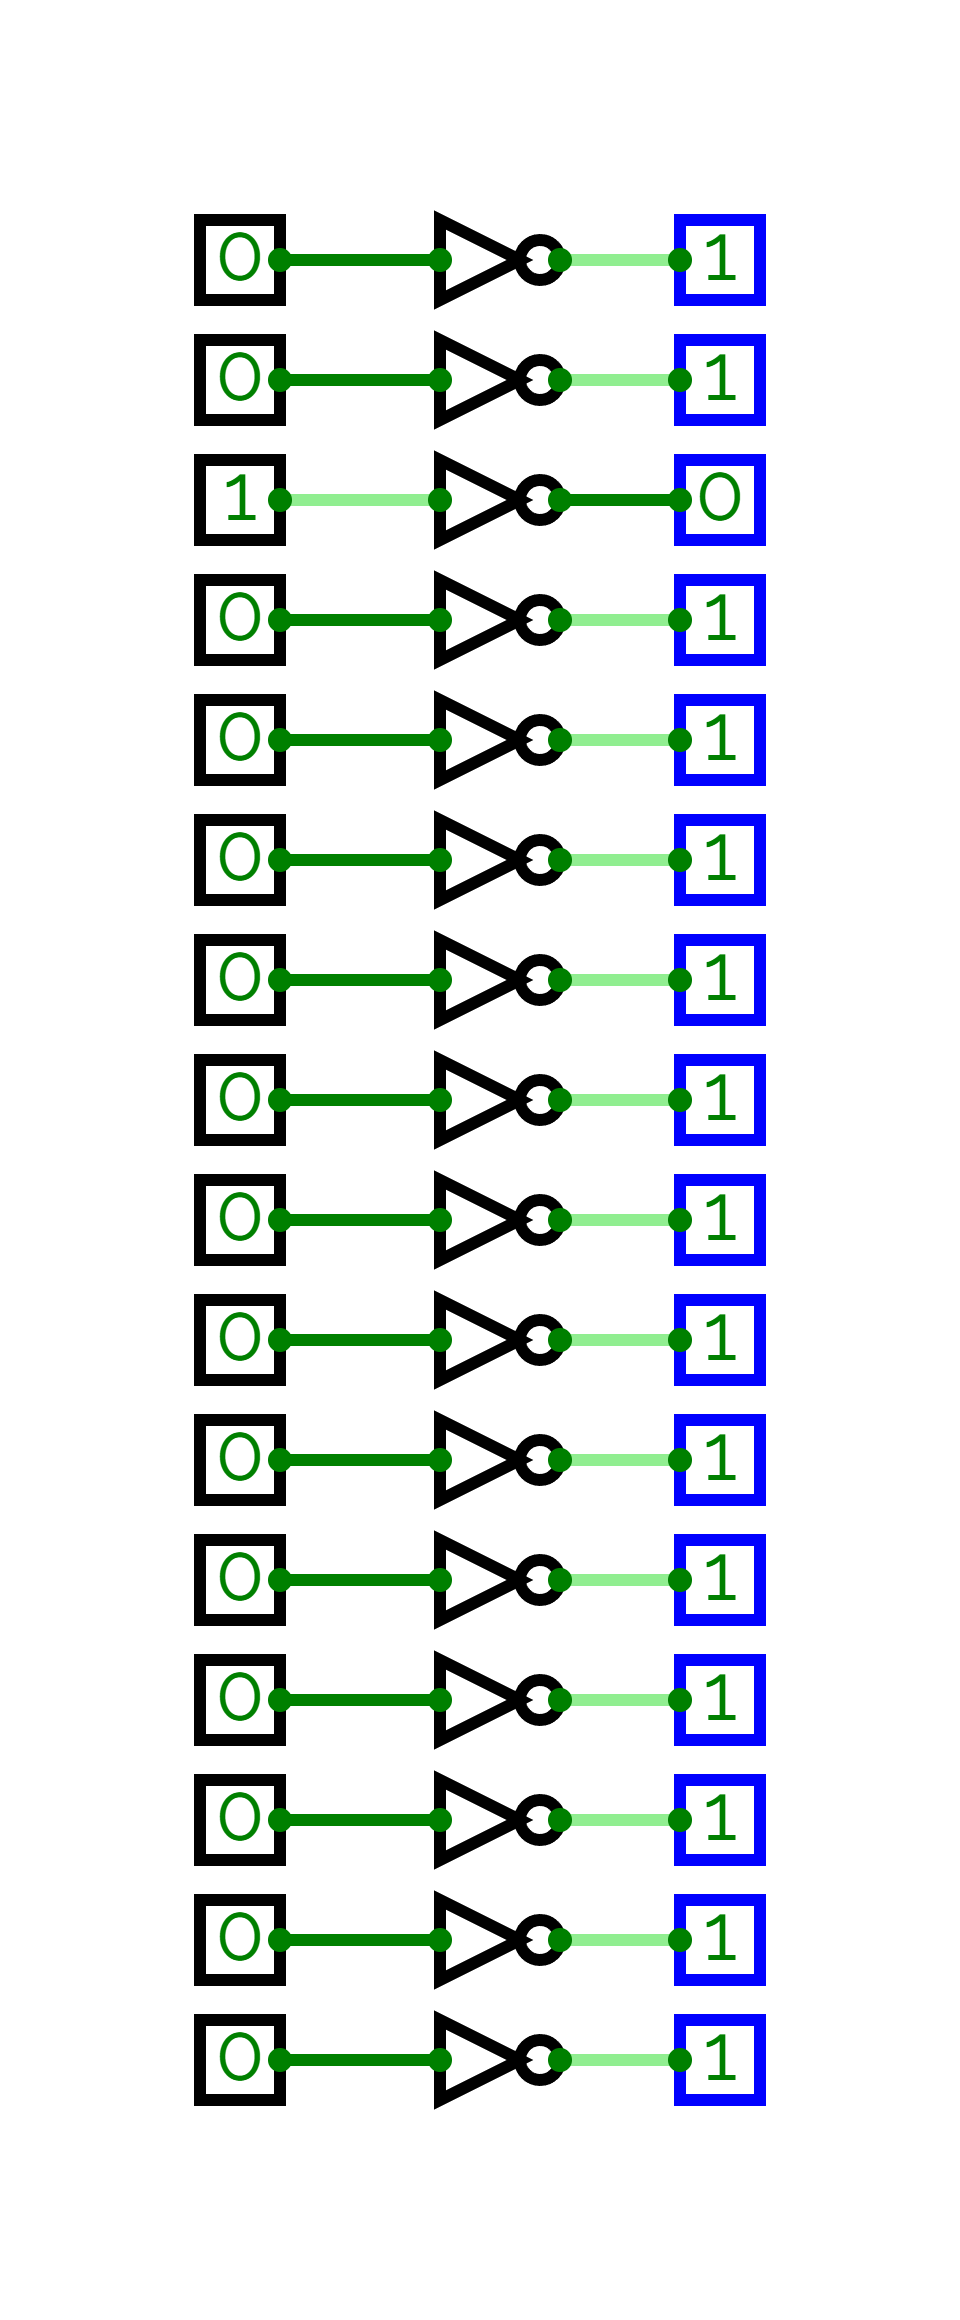
\includegraphics[width=0.4\textwidth]{CIRCUITOS/INT/NOT16_INT.png}
            \caption{Circuito interno de NOT16 \cite{circuitverse}}
            \label{fig:not16_int}
        \end{figure}
    \subsection{Esquema del circuito exterior}
        \begin{figure}[H]
            \centering
            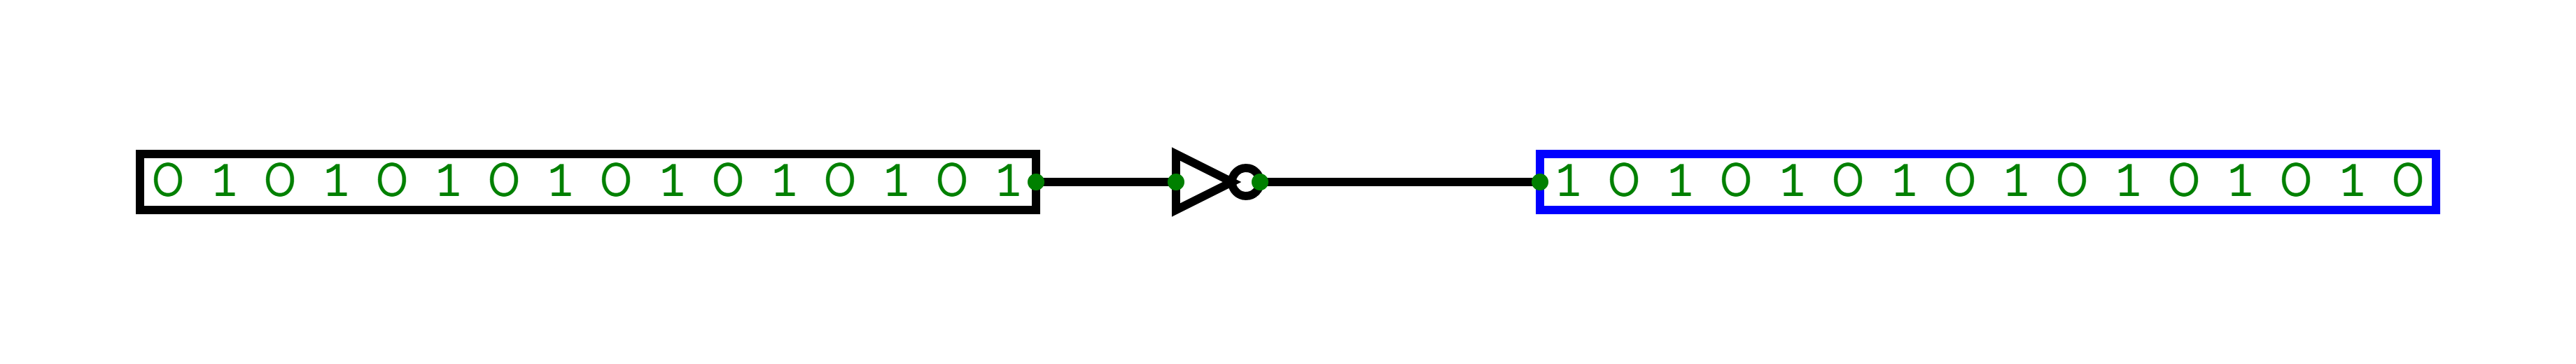
\includegraphics[width=1\textwidth]{CIRCUITOS/EXT/not16_ext.png}
            \caption{Circuito externo de NOT16 \cite{circuitverse}}
            \label{fig:not16_ext}
        \end{figure}
    \subsection{Implementación HDL}
        \begin{figure}[H]
            \centering
            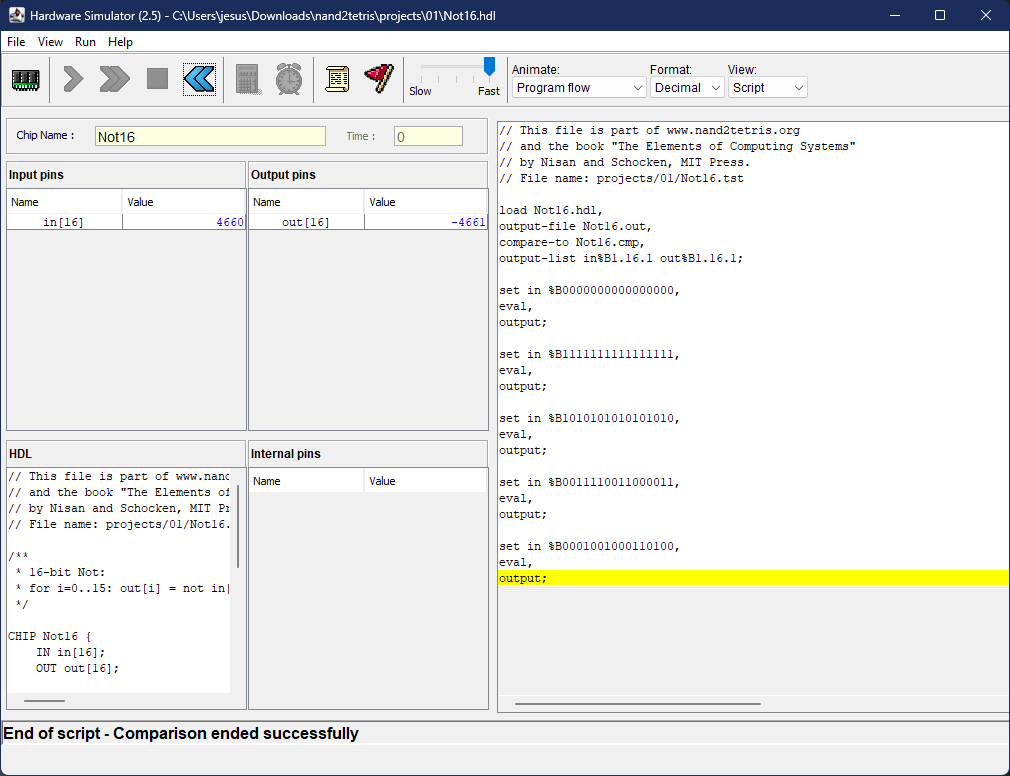
\includegraphics[width=0.75\textwidth]{CIRCUITOS/HDL/not16hdl.png}
            \caption{Test en Hardware Simulator de NOT16 \cite{nand2tetris}}
            \label{fig:hdlnot16}
        \end{figure}

        \subsubsection{Archivo HDL}
            \begin{lstlisting}
        CHIP Not16 {
            IN in[16];
            OUT out[16];
        
            PARTS:
            Not(in=in[0], out=out[0]);
            Not(in=in[1], out=out[1]);
            Not(in=in[2], out=out[2]);
            Not(in=in[3], out=out[3]);
            Not(in=in[4], out=out[4]);
            Not(in=in[5], out=out[5]);
            Not(in=in[6], out=out[6]);
            Not(in=in[7], out=out[7]);
            Not(in=in[8], out=out[8]);
            Not(in=in[9], out=out[9]);
            Not(in=in[10], out=out[10]);
            Not(in=in[11], out=out[11]);
            Not(in=in[12], out=out[12]);
            Not(in=in[13], out=out[13]);
            Not(in=in[14], out=out[14]);
            Not(in=in[15], out=out[15]);
        }
            \end{lstlisting}
    \newpage

%%%%%%%%%%%%%%%%%%%%%%%%%%%%%%%%%%%%%%%%%%%%%%%%%%%%%%%%%%%%%%%%%%%%%%%%%%
%%%%%%%%%%%%%%%%%%%%%%%%%%%%%%%%%%%%%%%%%%%%%%%%%%%%%%%%%%%%%%%%%%%%%%%%%%

\section{And16}
    Una puerta lógica de \textit{N}-bits And aplica una operación a cada uno de \textit{N}-pares conectados a sus dos buses inputs de \textit{N}-bits. \cite{nisan_nand2tetris_2005}
    \subsection{Tabla de verdad y explicación del circuito}
        \begin{table}[H]
        \centering
        \caption{Tabla de verdad de AND16}
        \label{tab:tab_and16}
        \resizebox{\textwidth}{!}{%
        \begin{tabular}{@{}lll@{}}
        \toprule
        \texttt{a}                & \texttt{b}                & \texttt{out}              \\ \midrule
        \texttt{0000000000000000} & \texttt{0000000000000000} & \texttt{0000000000000000} \\
        \texttt{0000000000000000} & \texttt{1111111111111111} & \texttt{0000000000000000} \\
        \texttt{1111111111111111} & \texttt{1111111111111111} & \texttt{1111111111111111} \\
        \texttt{1010101010101010} & \texttt{0101010101010101} & \texttt{0000000000000000} \\
        \texttt{0011110011000011} & \texttt{0000111111110000} & \texttt{0000110011000000} \\
        \texttt{0001001000110100} & \texttt{1001100001110110} & \texttt{0001000000110100} \\ \bottomrule
        \end{tabular}%
        }
        \end{table}

    \subsection{Esquema del circuito interior}
        \begin{figure}[H]
            \centering
            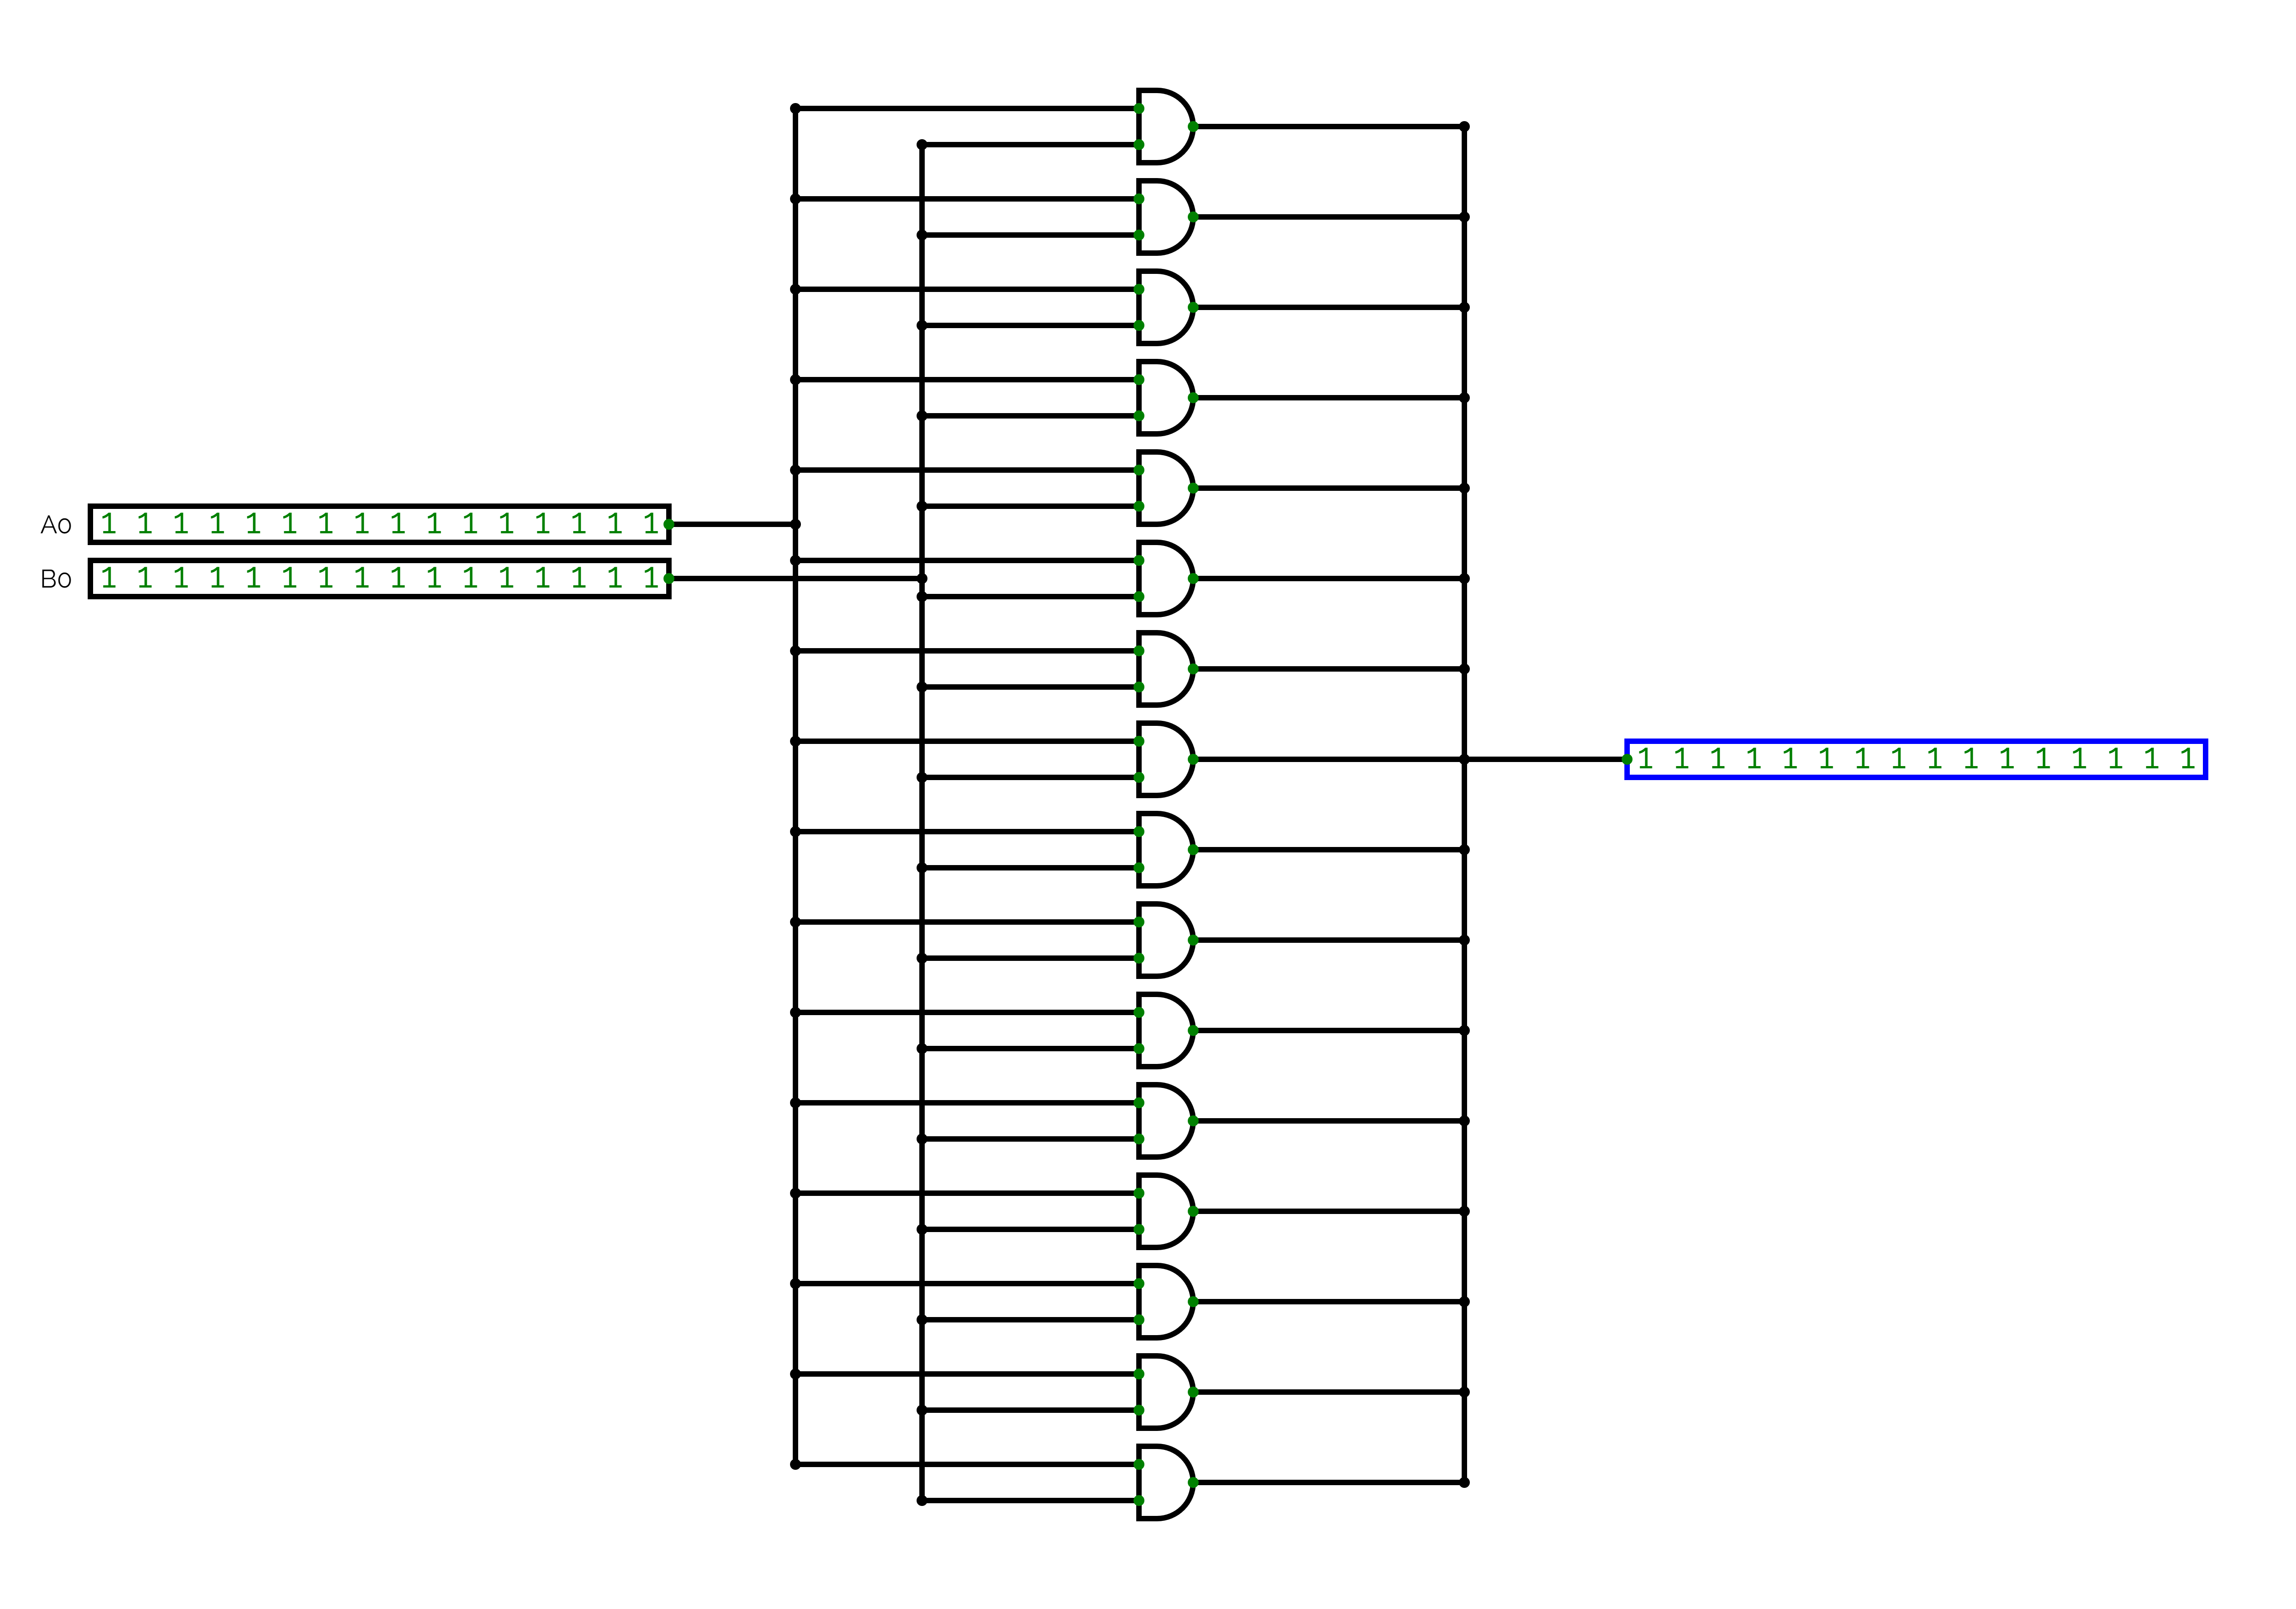
\includegraphics[width=\linewidth]{CIRCUITOS/INT/And16_int.png}
            \caption{Circuito interior de And16 \cite{circuitverse}}
            \label{fig:and16_int}
        \end{figure}
    \subsection{Esquema del circuito exterior}
        \begin{figure}[H]
            \centering
            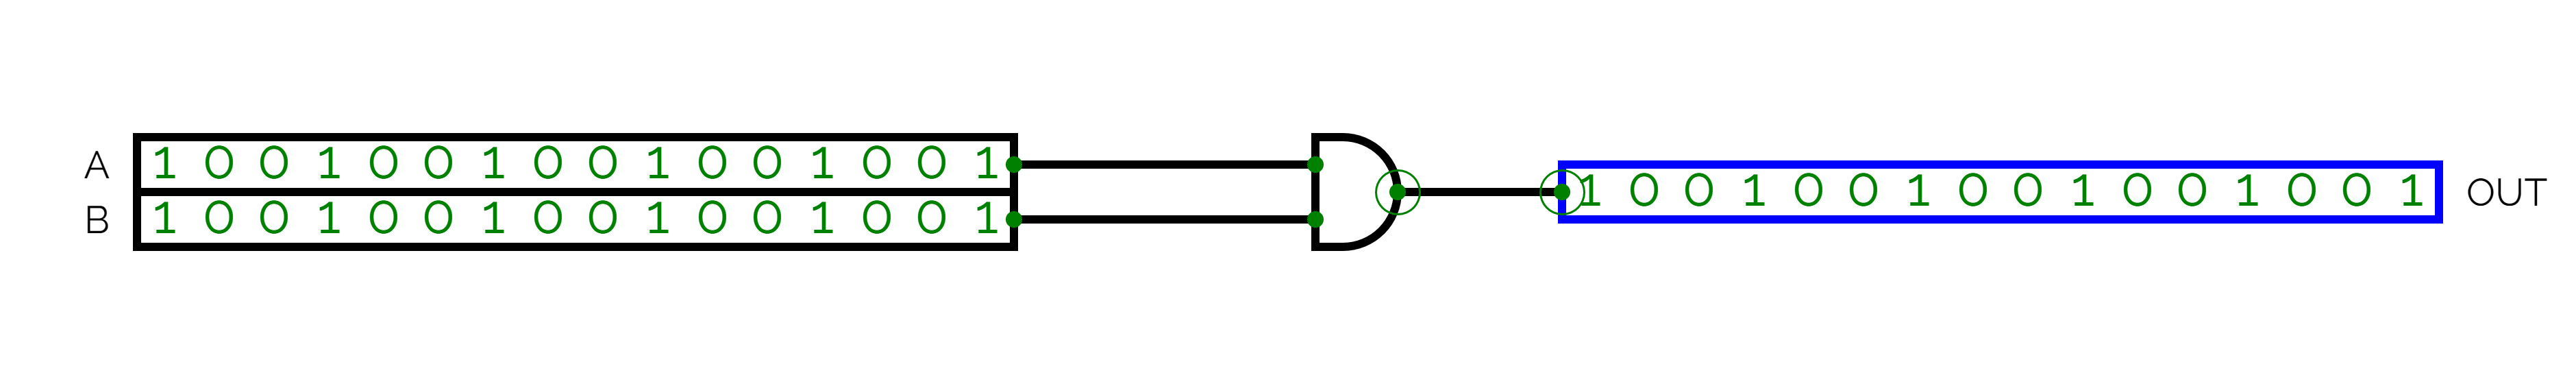
\includegraphics[width=\linewidth]{CIRCUITOS/EXT/and16_ext.png}
            \caption{Circuito exterior de And16 \cite{circuitverse}}
            \label{fig:and16_ext}
        \end{figure}
    \subsection{Implementación HDL}
        \begin{figure}[H]
            \centering
            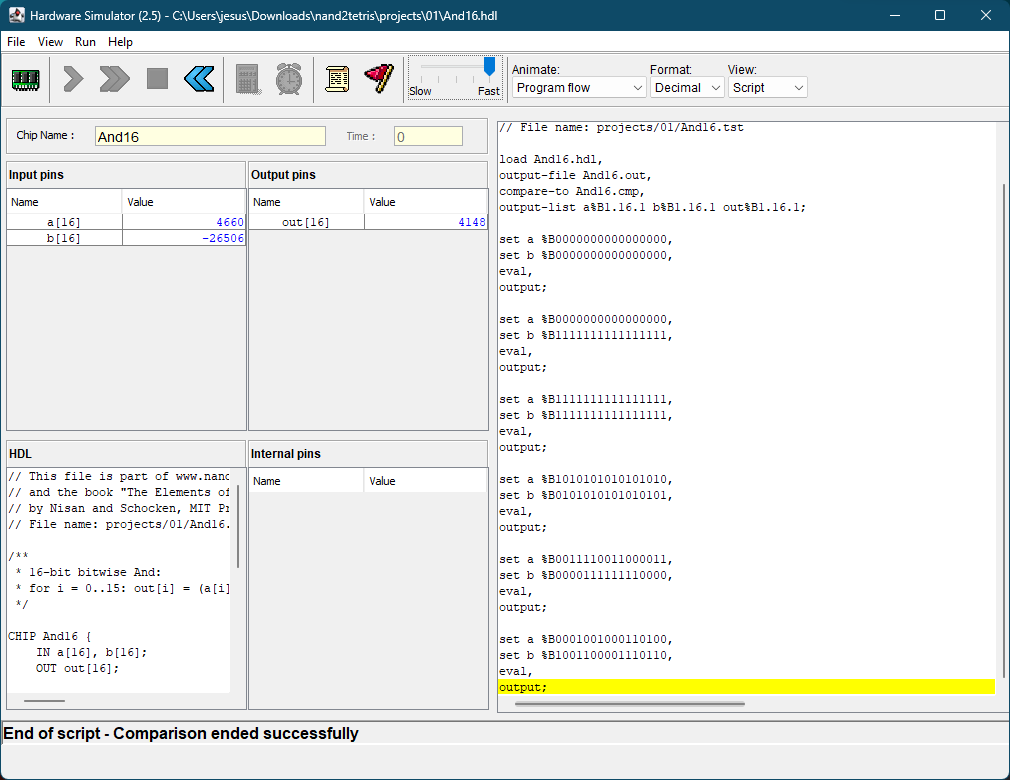
\includegraphics[width=0.75\linewidth]{CIRCUITOS/HDL/and16hdl.png}
            \caption{Test en Hardware Simulator de And16 \cite{nand2tetris}}
            \label{fig:hdland16}
        \end{figure}
        \subsubsection{Archivo HDL}
            \begin{lstlisting}
        CHIP And16 {
            IN a[16], b[16];
            OUT out[16];
        
            PARTS:
            And(a=a[0],b=b[0], out=out[0]);
            And(a=a[1],b=b[1], out=out[1]);
            And(a=a[2],b=b[2], out=out[2]);
            And(a=a[3],b=b[3], out=out[3]);
            And(a=a[4],b=b[4], out=out[4]);
            And(a=a[5],b=b[5], out=out[5]);
            And(a=a[6],b=b[6], out=out[6]);
            And(a=a[7],b=b[7], out=out[7]);
            And(a=a[8],b=b[8], out=out[8]);
            And(a=a[9],b=b[9], out=out[9]);
            And(a=a[10],b=b[10],out=out[10]);
            And(a=a[11],b=b[11],out=out[11]);
            And(a=a[12],b=b[12],out=out[12]);
            And(a=a[13],b=b[13],out=out[13]);
            And(a=a[14],b=b[14],out=out[14]);
            And(a=a[15],b=b[15],out=out[15]);
        }
            \end{lstlisting}
    \newpage
    
%%%%%%%%%%%%%%%%%%%%%%%%%%%%%%%%%%%%%%%%%%%%%%%%%%%%%%%%%%%%%%%%%%%%%%%%%%
%%%%%%%%%%%%%%%%%%%%%%%%%%%%%%%%%%%%%%%%%%%%%%%%%%%%%%%%%%%%%%%%%%%%%%%%%%

\section{Or16}
    \subsection{Tabla de verdad y explicación del circuito}
    La puerta lógica Or de \textit{N}-bits aplica una operación booleana de tipo Or a cada uno de sus inputs pares de \textit{N}-bits. \cite{nisan_nand2tetris_2005}
        \begin{table}[H]
        \centering
        \caption{Tabla de verdad de OR16}
        \label{tab:tab_or16}
        \resizebox{\textwidth}{!}{%
        \begin{tabular}{@{}lll@{}}
        \toprule
        \texttt{a}                & \texttt{b}                & \texttt{out}              \\ \midrule
        \texttt{0000000000000000} & \texttt{0000000000000000} & \texttt{0000000000000000} \\
        \texttt{0000000000000000} & \texttt{1111111111111111} & \texttt{1111111111111111} \\
        \texttt{1111111111111111} & \texttt{1111111111111111} & \texttt{1111111111111111} \\
        \texttt{1010101010101010} & \texttt{0101010101010101} & \texttt{1111111111111111} \\
        \texttt{0011110011000011} & \texttt{0000111111110000} & \texttt{0011111111110011} \\
        \texttt{0001001000110100} & \texttt{1001100001110110} & \texttt{1001101001110110} \\ \bottomrule
        \end{tabular}%
        }
        \end{table}
        
    \subsection{Esquema del circuito interior}
        \begin{figure}[H]
            \centering
            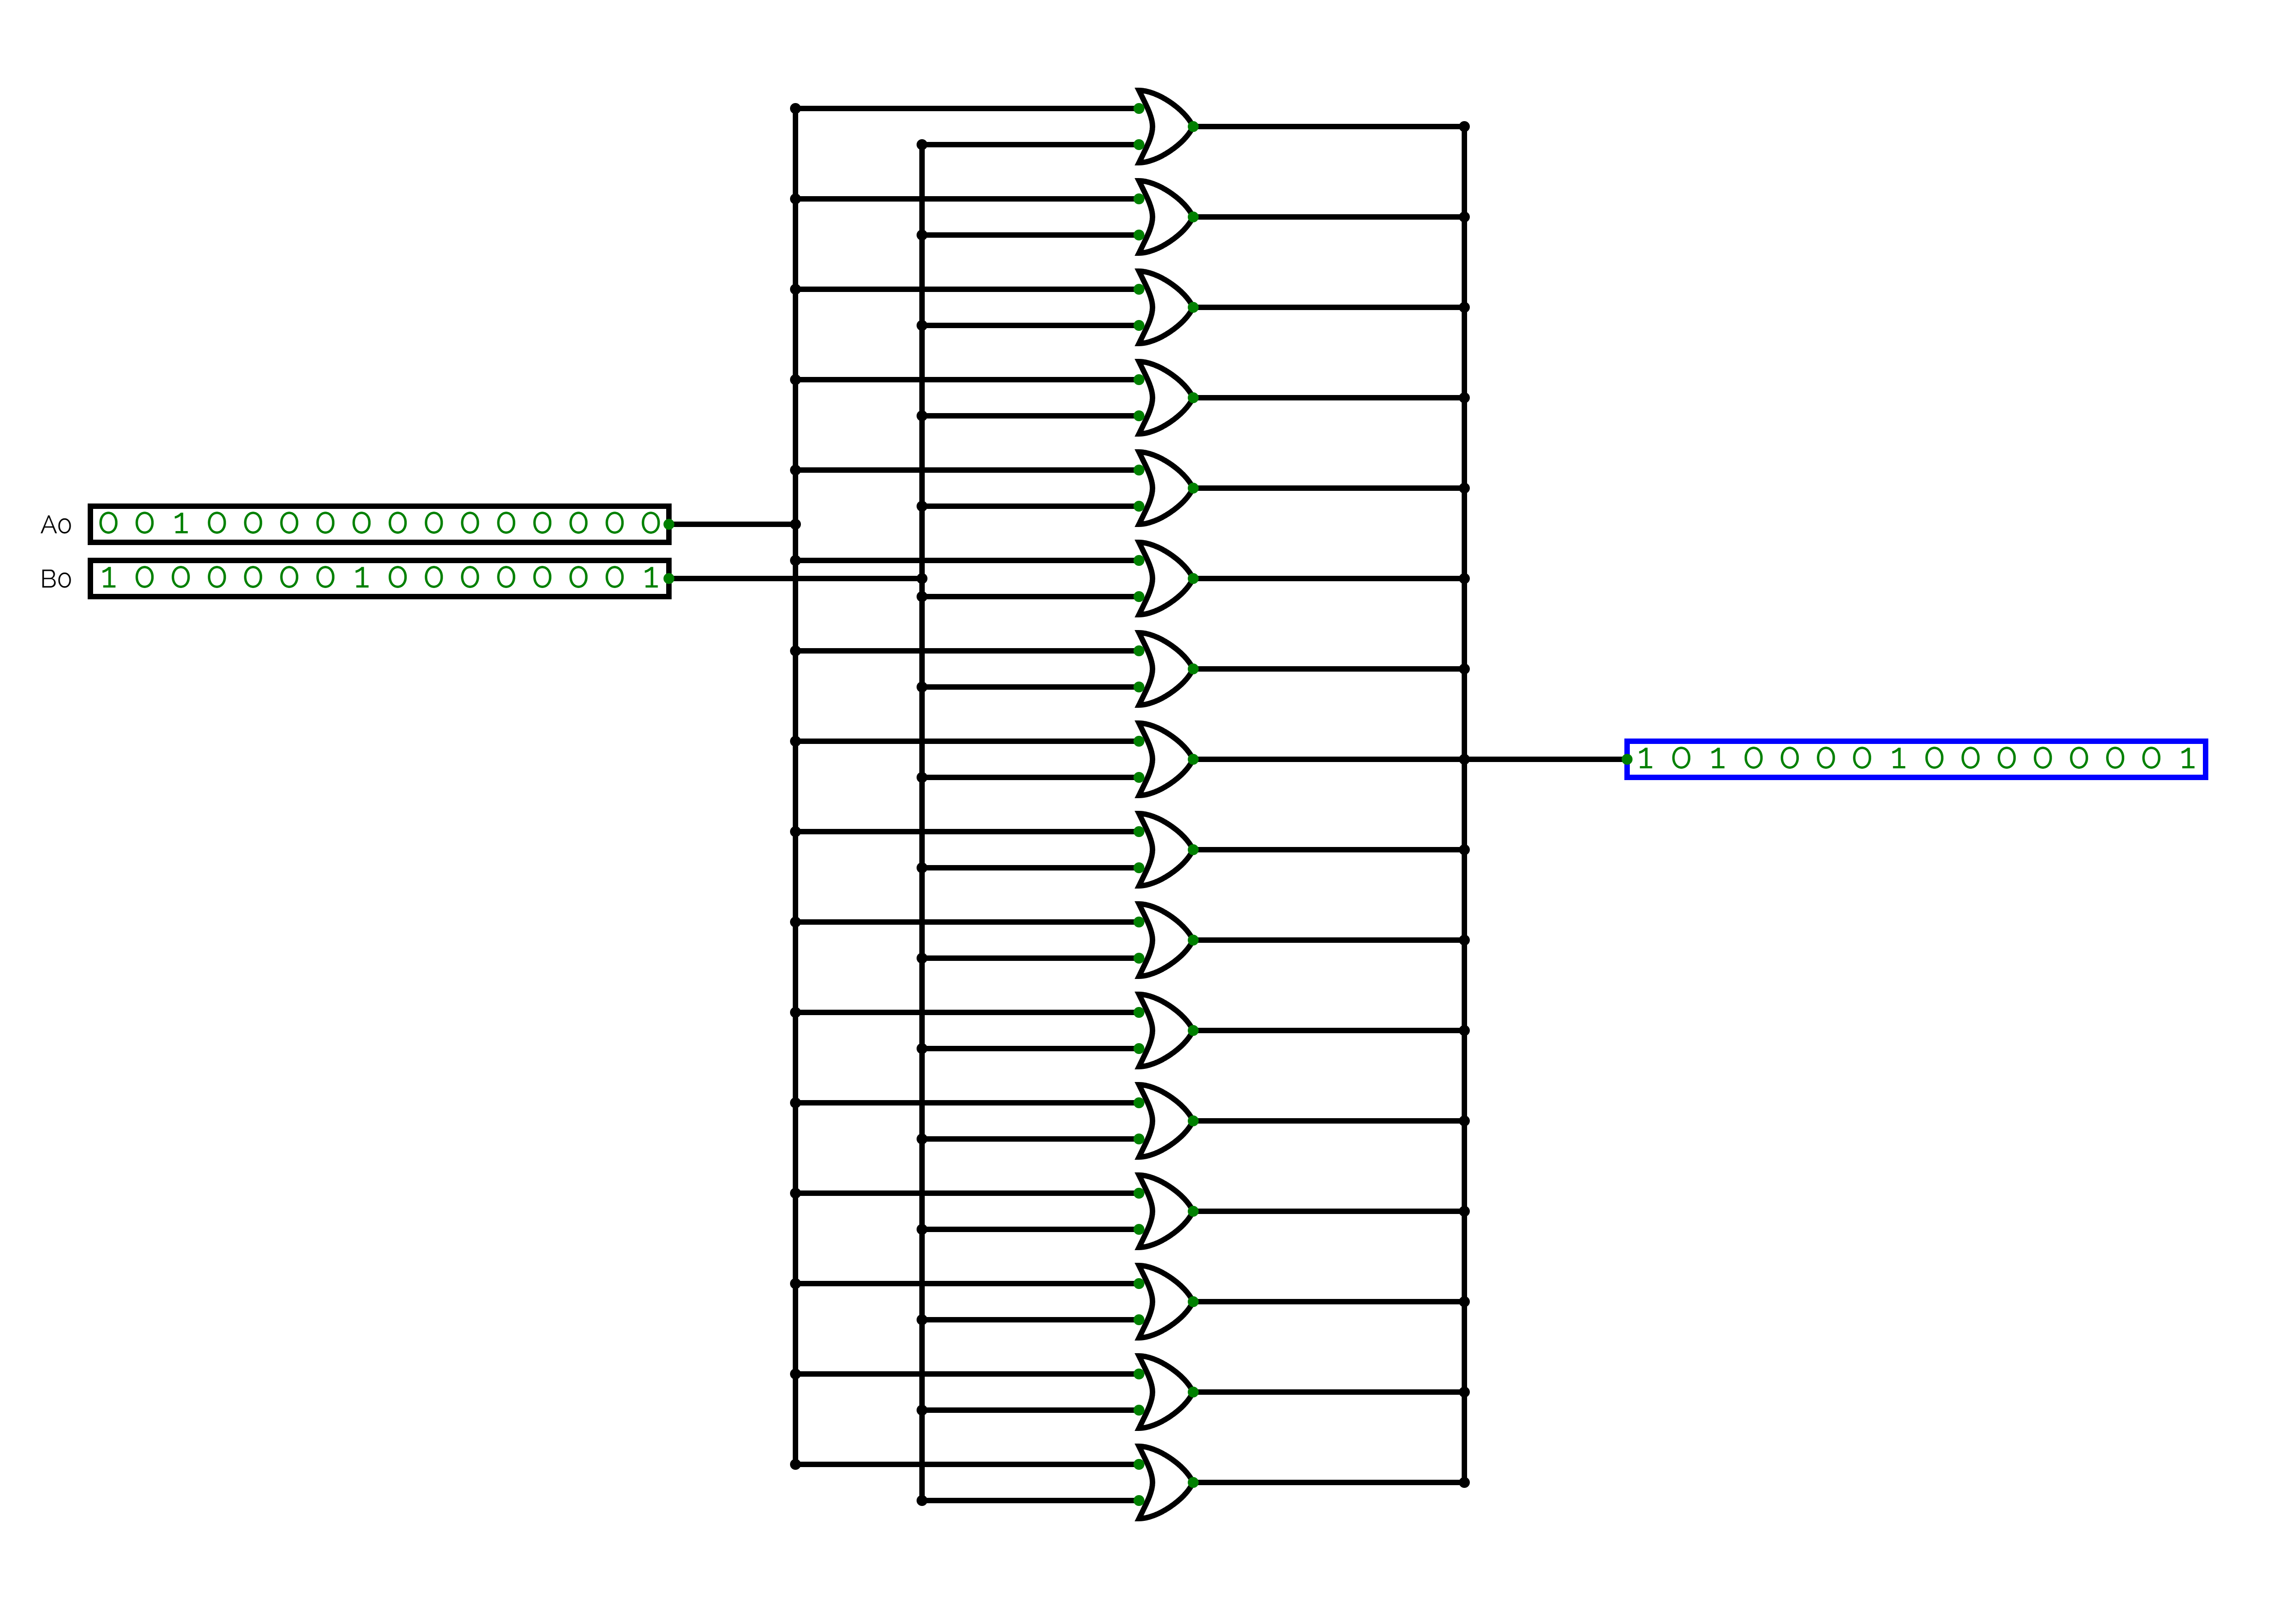
\includegraphics[width=1\textwidth]{CIRCUITOS/INT/OR16_int.png}
            \caption{Circuito interior de Or16 \cite{circuitverse}}
            \label{fig:or16_int}
        \end{figure}
    \subsection{Esquema del circuito exterior}
        \begin{figure}[H]
            \centering
            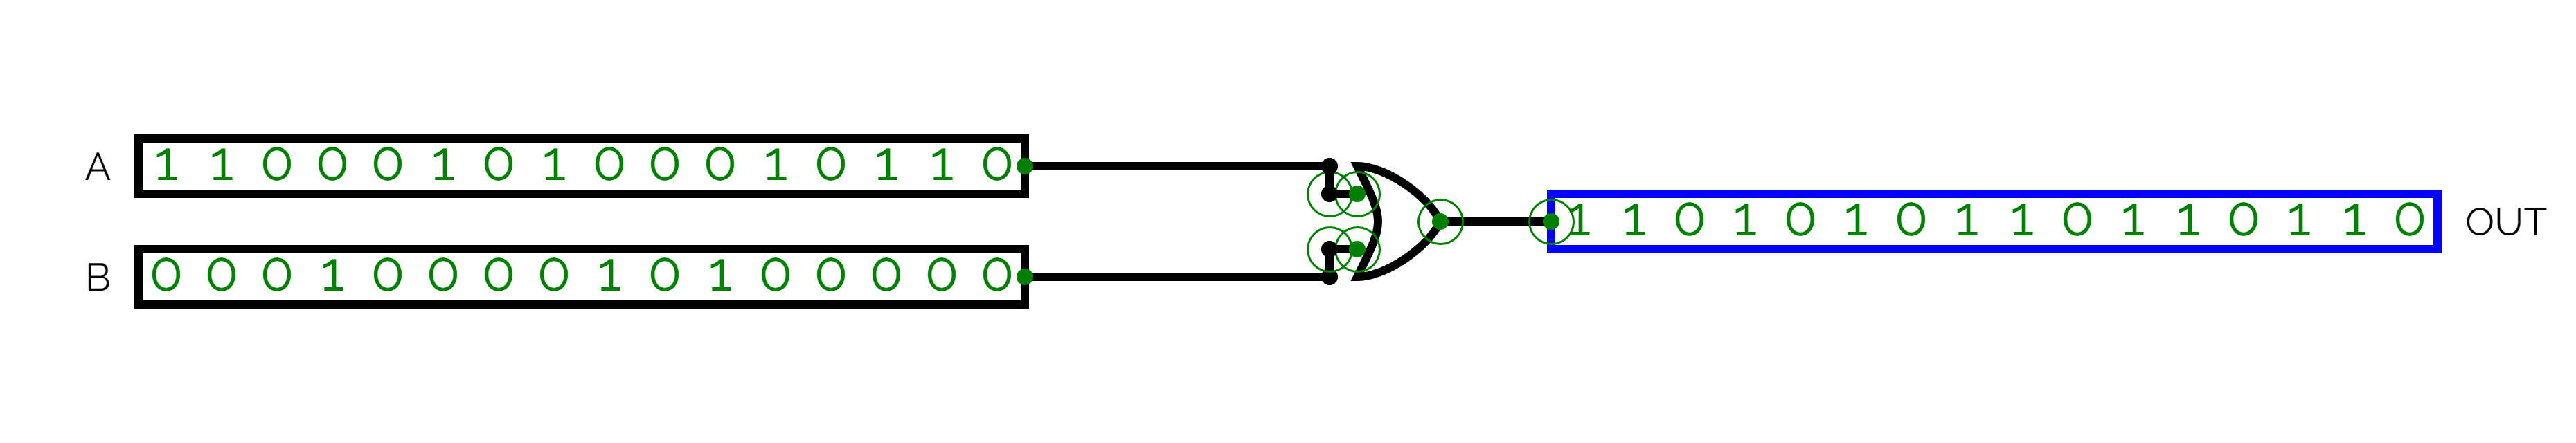
\includegraphics[width=1\textwidth]{CIRCUITOS/EXT/OR16_ext.png}
            \caption{Circuito exterior de Or16 \cite{circuitverse}}
            \label{fig:or16_ext}
        \end{figure}
    \subsection{Implementación HDL}
        \begin{figure}[H]
            \centering
            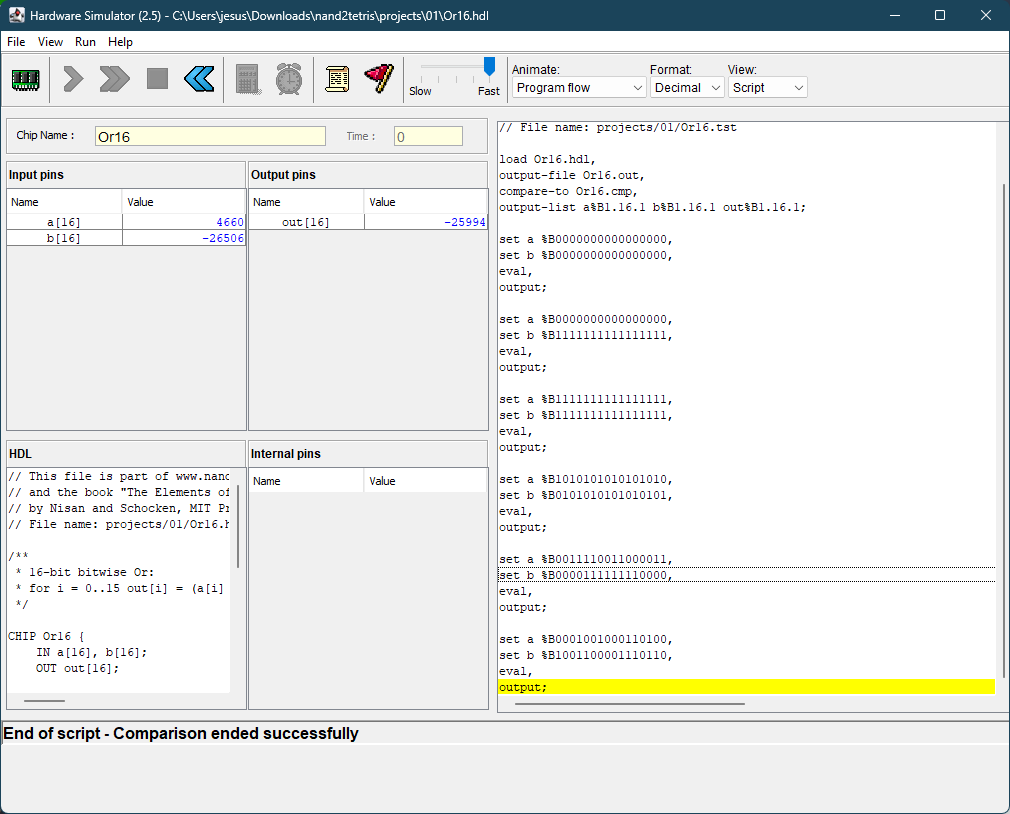
\includegraphics[width=0.75\linewidth]{CIRCUITOS//HDL/or16hdl.png}
            \caption{Test en Hardware Simulator de Or16 \cite{nand2tetris}}
            \label{fig:hdlor16}
        \end{figure}
        \subsubsection{Archivo HDL}
            \begin{lstlisting}
        CHIP Or16 {
            IN a[16], b[16];
            OUT out[16];
        
            PARTS:
                Or(a=a[0], b=b[0], out=out[0]);
                Or(a=a[1], b=b[1], out=out[1]);
                Or(a=a[2], b=b[2], out=out[2]);
                Or(a=a[3], b=b[3], out=out[3]);
                Or(a=a[4], b=b[4], out=out[4]);
                Or(a=a[5], b=b[5], out=out[5]);
                Or(a=a[6], b=b[6], out=out[6]);
                Or(a=a[7], b=b[7], out=out[7]);
                Or(a=a[8], b=b[8], out=out[8]);
                Or(a=a[9], b=b[9], out=out[9]);
                Or(a=a[10], b=b[10], out=out[10]);
                Or(a=a[11], b=b[11], out=out[11]);
                Or(a=a[12], b=b[12], out=out[12]);
                Or(a=a[13], b=b[13], out=out[13]);
                Or(a=a[14], b=b[14], out=out[14]);
                Or(a=a[15], b=b[15], out=out[15]);
        }
            \end{lstlisting}  
    \newpage

%%%%%%%%%%%%%%%%%%%%%%%%%%%%%%%%%%%%%%%%%%%%%%%%%%%%%%%%%%%%%%%%%%%%%%%%%%
%%%%%%%%%%%%%%%%%%%%%%%%%%%%%%%%%%%%%%%%%%%%%%%%%%%%%%%%%%%%%%%%%%%%%%%%%%

\section{Mux16}
    \subsection{Tabla de verdad y explicación del circuito}
        Un multiplexador (Mux\textit{X}bits) de \textit{N}-bits, se comporta de manera parecida a un Mux exceptuando en que sus dos inputs son de \textit{N}-bits de ancho (16 en este caso). \cite{nisan_nand2tetris_2005}
        \begin{table}[H]
        \centering
        \caption{Tabla de verdad de MUX16}
        \label{tab:tab_mux16}
        \resizebox{\columnwidth}{!}{%
        \begin{tabular}{@{}llll@{}}
        \toprule
        \texttt{a}                & \texttt{b}                & \texttt{sel} & \texttt{out}              \\ \midrule
        \texttt{0000000000000000} & \texttt{0000000000000000} & \texttt{0}   & \texttt{0000000000000000} \\
        \texttt{0000000000000000} & \texttt{0000000000000000} & \texttt{1}   & \texttt{0000000000000000} \\
        \texttt{0000000000000000} & \texttt{0001001000110100} & \texttt{0}   & \texttt{0000000000000000} \\
        \texttt{0000000000000000} & \texttt{0001001000110100} & \texttt{1}   & \texttt{0001001000110100} \\
        \texttt{1001100001110110} & \texttt{0000000000000000} & \texttt{0}   & \texttt{1001100001110110} \\
        \texttt{1001100001110110} & \texttt{0000000000000000} & \texttt{1}   & \texttt{0000000000000000} \\
        \texttt{1010101010101010} & \texttt{0101010101010101} & \texttt{0}   & \texttt{1010101010101010} \\
        \texttt{1010101010101010} & \texttt{0101010101010101} & \texttt{1}   & \texttt{0101010101010101} \\ \bottomrule
        \end{tabular}%
        }
        \end{table}

    \subsection{Esquema del circuito interior}
        \begin{figure}[H]
            \centering
            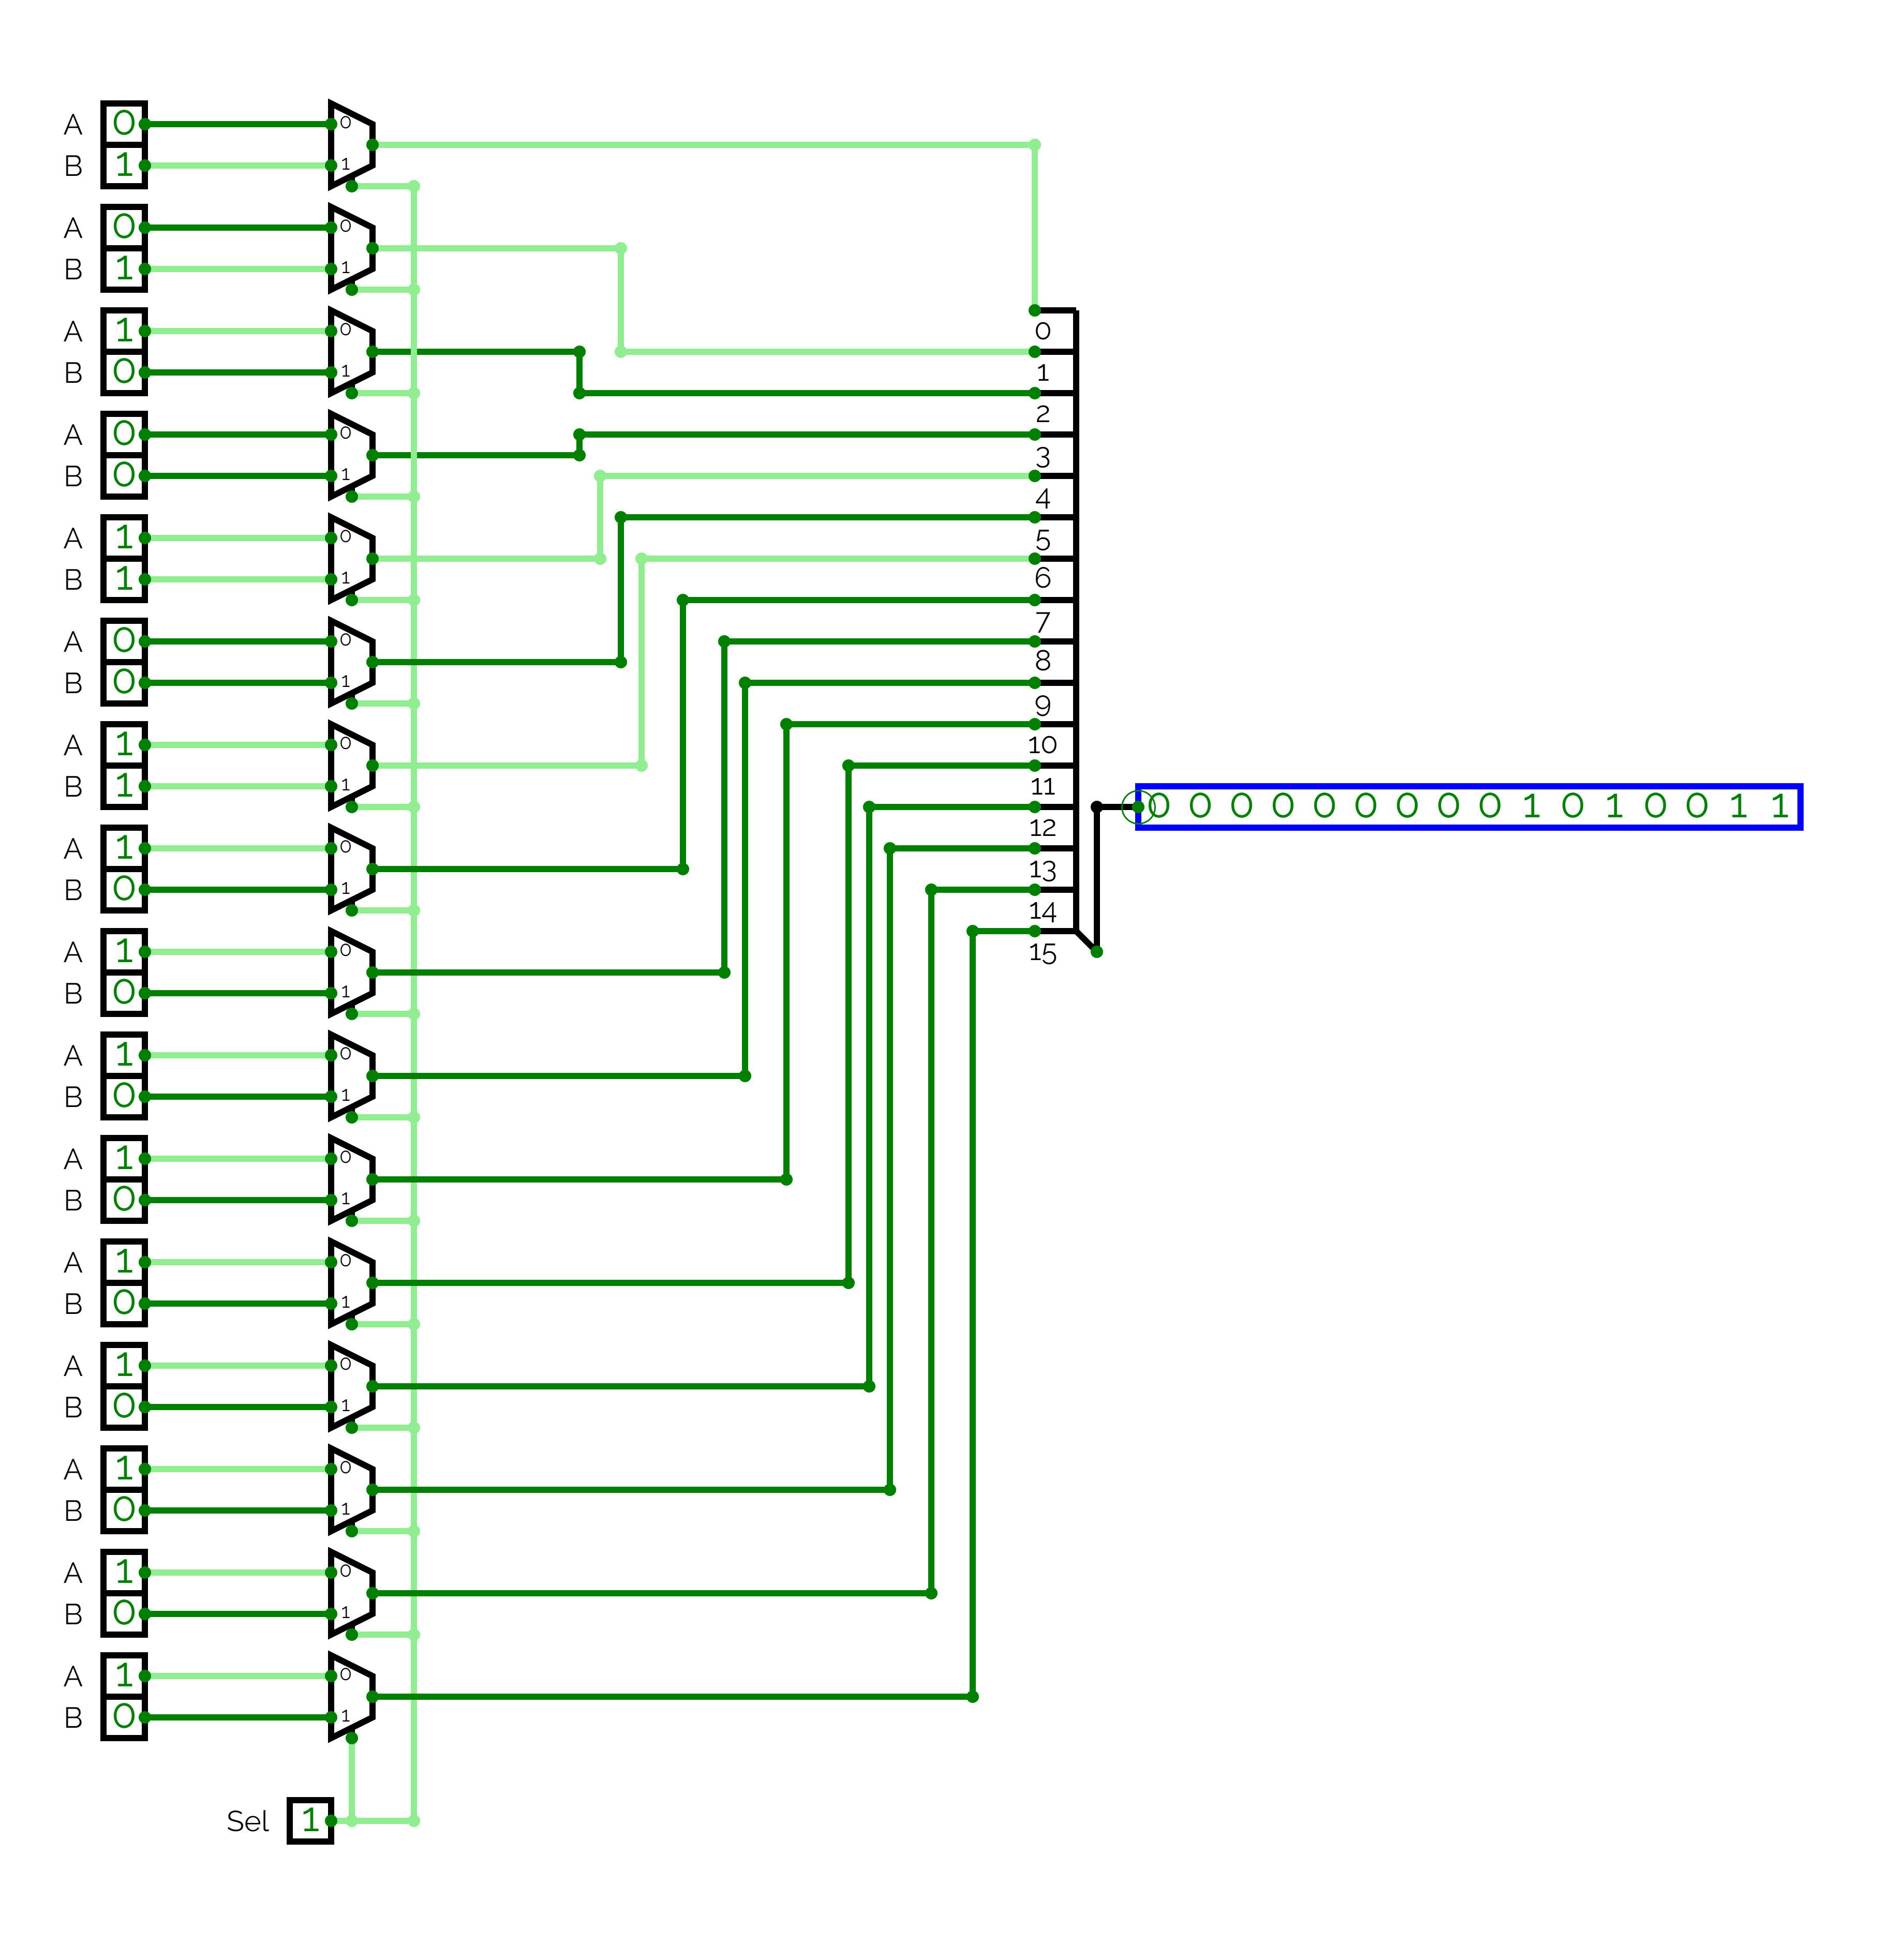
\includegraphics[width=1\textwidth]{CIRCUITOS/INT/Mux16_int.png}            
            \caption{Circuito interior de Mux16 \cite{circuitverse}}
            \label{fig:mux16_int}
        \end{figure}
    \subsection{Esquema del circuito exterior}
        \begin{figure}[H]
            \centering
            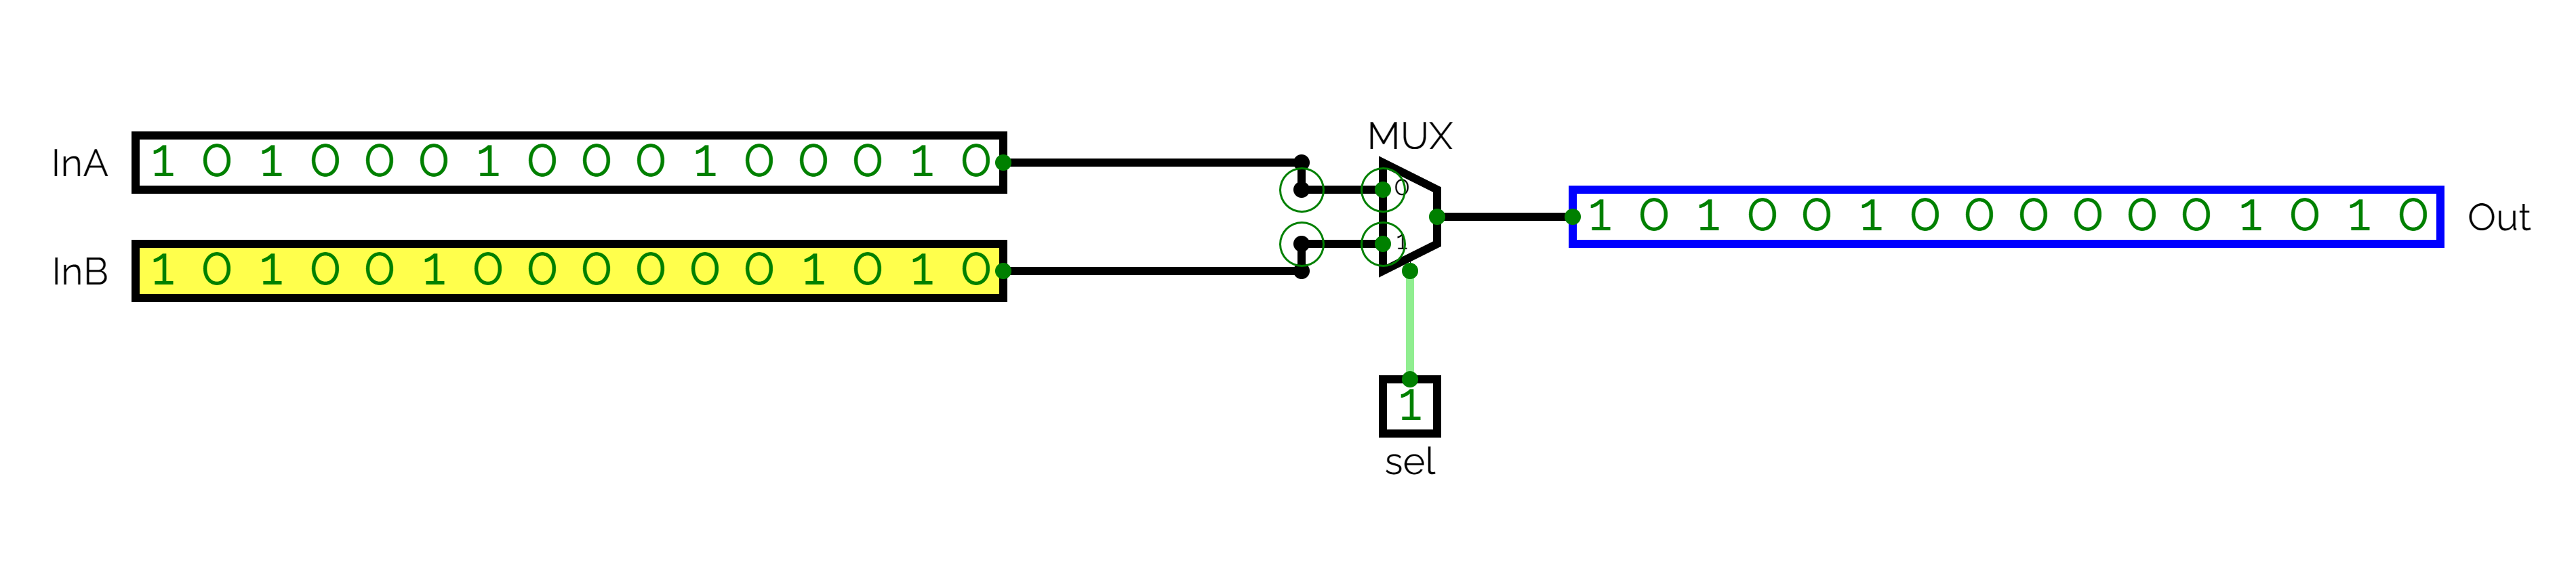
\includegraphics[width=1\textwidth]{CIRCUITOS/EXT/Mux16_ext1.png}            
            \caption{Circuito exterior de Mux16 \cite{circuitverse}}
            \label{fig:mux16_ext}
        \end{figure}
    \subsection{Implementación HDL}
        \begin{figure}[H]
            \centering
            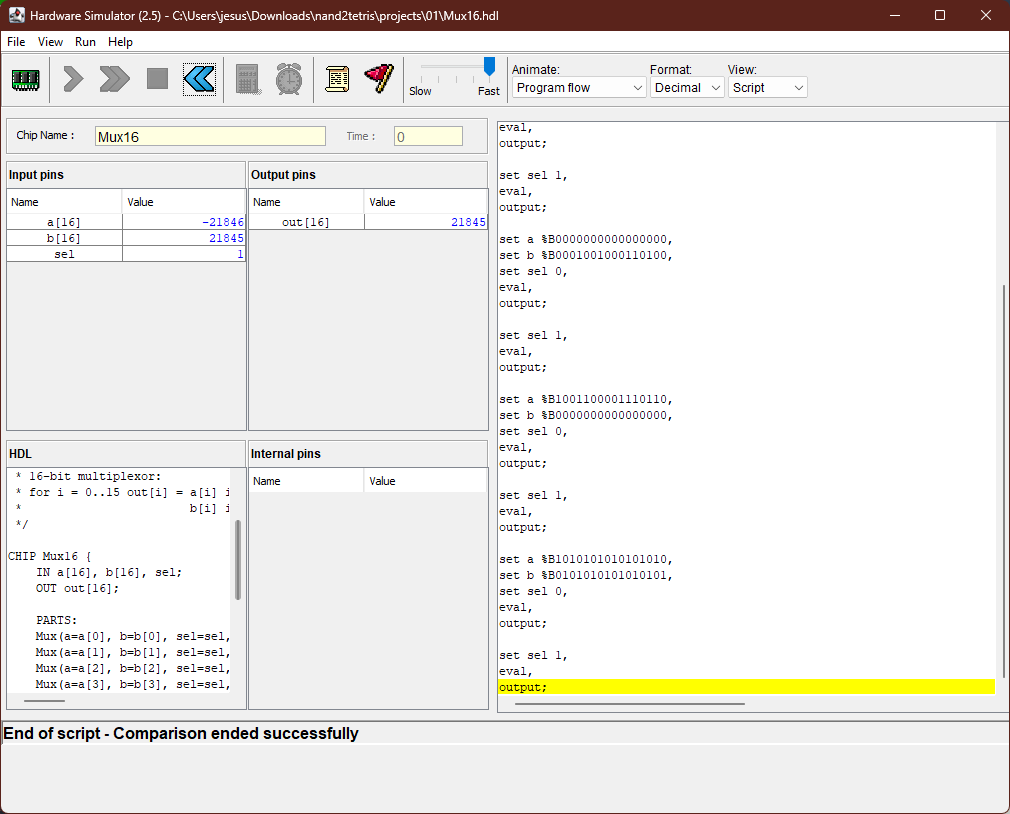
\includegraphics[width=0.75\linewidth]{CIRCUITOS//HDL/mux16hdl.png}
            \caption{Test en Hardware Simulator de Mux16 \cite{nand2tetris}}
            \label{fig:hdlmux16}
        \end{figure}
        \subsubsection{Archivo HDL}
            \begin{lstlisting}
                
        CHIP Mux16 {
            IN a[16], b[16], sel;
            OUT out[16];
        
            PARTS:
            Mux(a=a[0], b=b[0], sel=sel, out=out[0]);
            Mux(a=a[1], b=b[1], sel=sel, out=out[1]);
            Mux(a=a[2], b=b[2], sel=sel, out=out[2]);
            Mux(a=a[3], b=b[3], sel=sel, out=out[3]);
            Mux(a=a[4], b=b[4], sel=sel, out=out[4]);
            Mux(a=a[5], b=b[5], sel=sel, out=out[5]);
            Mux(a=a[6], b=b[6], sel=sel, out=out[6]);
            Mux(a=a[7], b=b[7], sel=sel, out=out[7]);
            Mux(a=a[8], b=b[8], sel=sel, out=out[8]);
            Mux(a=a[9], b=b[9], sel=sel, out=out[9]);
            Mux(a=a[10], b=b[10], sel=sel, out=out[10]);
            Mux(a=a[11], b=b[11], sel=sel, out=out[11]);
            Mux(a=a[12], b=b[12], sel=sel, out=out[12]);
            Mux(a=a[13], b=b[13], sel=sel, out=out[13]);
            Mux(a=a[14], b=b[14], sel=sel, out=out[14]);
            Mux(a=a[15], b=b[15], sel=sel, out=out[15]);
        }
            \end{lstlisting}
    \newpage

%%%%%%%%%%%%%%%%%%%%%%%%%%%%%%%%%%%%%%%%%%%%%%%%%%%%%%%%%%%%%%%%%%%%%%%%%%
%%%%%%%%%%%%%%%%%%%%%%%%%%%%%%%%%%%%%%%%%%%%%%%%%%%%%%%%%%%%%%%%%%%%%%%%%%

\section{DMux4Way (DMuxi1o4b1)} \label{dmux4label}
    \subsection{Tabla de verdad y explicación del circuito}
        Un demultiplexador de \textit{M}-vías y \textit{N}-bits guía a 1 bit desde su input de un 1 bit, hasta uno de los posibles outputs de \textit{N}-bits. Cuya selección se realiza mediante una colección de bits \textit{k}, cuya fórmula es $k = log_{2}m$. \label{dmux4text} \cite{nisan_nand2tetris_2005}
        \begin{table}[H]
        \centering
        \caption{Tabla de verdad de DMUX4WAY}
        \label{tab:tab_dmux4way}
        \resizebox{0.9\columnwidth}{!}{%
        \begin{tabular}{@{}llllll@{}}
        \toprule
        \texttt{in} & \texttt{sel} & \texttt{a} & \texttt{b} & \texttt{c} & \texttt{d} \\ \midrule
        \texttt{0}  & \texttt{00}  & \texttt{0} & \texttt{0} & \texttt{0} & \texttt{0} \\
        \texttt{0}  & \texttt{01}  & \texttt{0} & \texttt{0} & \texttt{0} & \texttt{0} \\
        \texttt{0}  & \texttt{10}  & \texttt{0} & \texttt{0} & \texttt{0} & \texttt{0} \\
        \texttt{0}  & \texttt{11}  & \texttt{0} & \texttt{0} & \texttt{0} & \texttt{0} \\
        \texttt{1}  & \texttt{00}  & \texttt{1} & \texttt{0} & \texttt{0} & \texttt{0} \\
        \texttt{1}  & \texttt{01}  & \texttt{0} & \texttt{1} & \texttt{0} & \texttt{0} \\
        \texttt{1}  & \texttt{10}  & \texttt{0} & \texttt{0} & \texttt{1} & \texttt{0} \\
        \texttt{1}  & \texttt{11}  & \texttt{0} & \texttt{0} & \texttt{0} & \texttt{1} \\ \bottomrule
        \end{tabular}%
        }
        \end{table}

    \subsection{Esquema del circuito interior}
        \begin{figure}[H]
            \centering
            \includegraphics[width=1\textwidth]{CIRCUITOS/INT/Dmux4way_int.png}            
            \caption{Circuito interior de DMux4Way \cite{circuitverse}}
            \label{fig:dmux4way_int}
        \end{figure}
        
    \subsection{Esquema del circuito exterior}
        \begin{figure}[H]
            \centering
            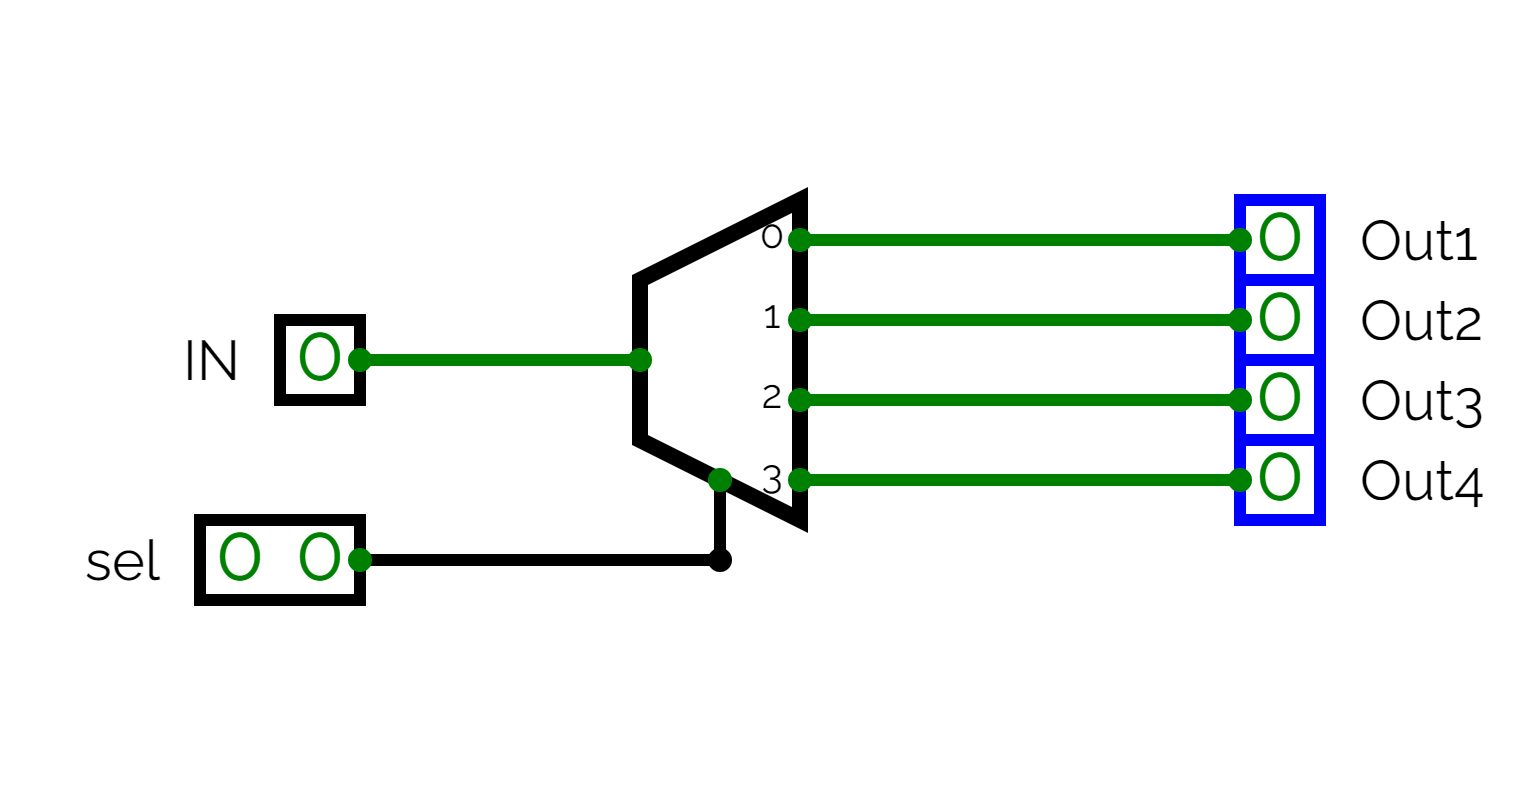
\includegraphics[width=1\textwidth]{CIRCUITOS/EXT/DMUX4WAY_ext.png}            
            \caption{Circuito exterior de DMux4Way \cite{circuitverse}}
            \label{fig:dmux4way_ext}
        \end{figure}
    \subsection{Implementación HDL}
        \begin{figure}[H]
            \centering
            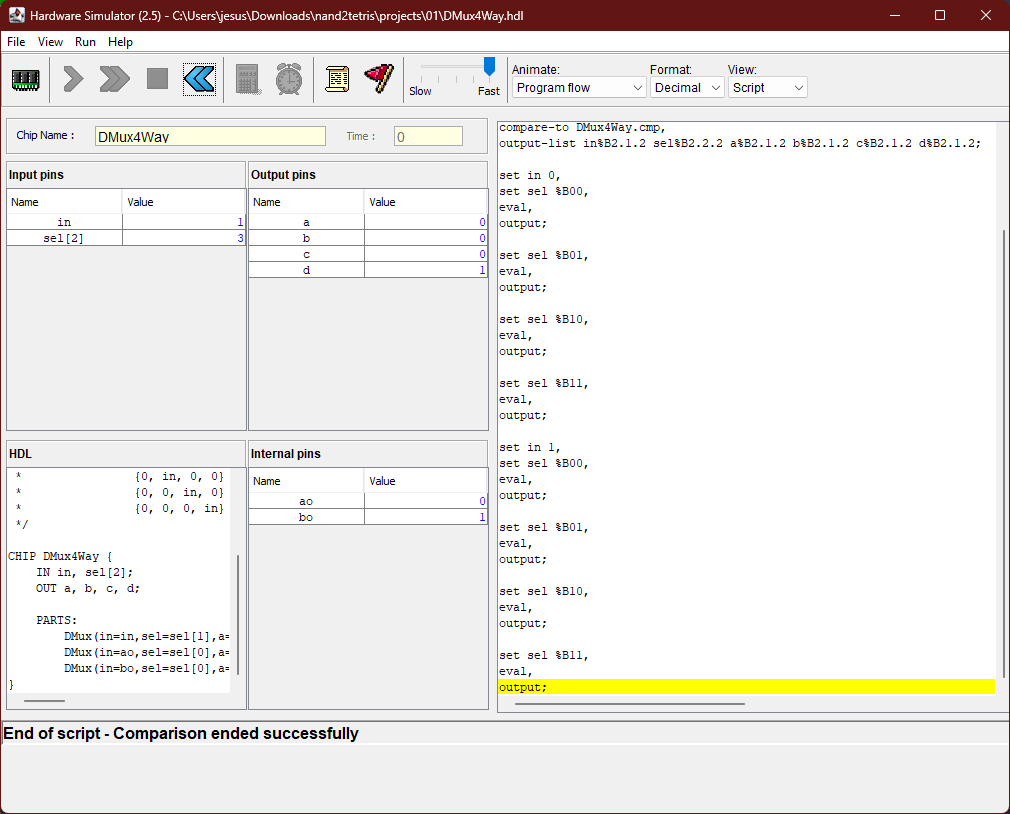
\includegraphics[width=0.75\linewidth]{CIRCUITOS//HDL/dmux4way.png}
            \caption{Test en Hardware Simulator de DMux4Way \cite{nand2tetris}}
            \label{fig:hdldmux4way}
        \end{figure}
        \subsubsection{Archivo HDL}
            \begin{lstlisting}
        CHIP DMux4Way {
            IN in, sel[2];
            OUT a, b, c, d;
        
            PARTS:
                DMux(in=in,sel=sel[1],a=ao,b=bo);
                DMux(in=ao,sel=sel[0],a=a,b=b);
                DMux(in=bo,sel=sel[0],a=c,b=d);
        }
            \end{lstlisting}
    \newpage

%%%%%%%%%%%%%%%%%%%%%%%%%%%%%%%%%%%%%%%%%%%%%%%%%%%%%%%%%%%%%%%%%%%%%%%%%%
%%%%%%%%%%%%%%%%%%%%%%%%%%%%%%%%%%%%%%%%%%%%%%%%%%%%%%%%%%%%%%%%%%%%%%%%%%

\section{DMux8Way (DMuxi1o8b1)}
    \subsection{Tabla de verdad y explicación del circuito}
        Mismo concepto usado en \ref{dmux4label}, exceptuando que en vez de 4 outputs \ref{dmux4text}, se usan 8 outputs. \cite{nisan_nand2tetris_2005}

        \begin{table}[H]
        \centering
        \caption{Tabla de verdad de DMUX8WAY}
        \label{tab:tab_dmux8way}
        \resizebox{0.8\columnwidth}{!}{%
        \begin{tabular}{@{}llllllllll@{}}
        \toprule
        \texttt{in} & \texttt{sel} & \texttt{a} & \texttt{b} & \texttt{c} & \texttt{d} & \texttt{e} & \texttt{f} & \texttt{g} & \texttt{h} \\ \midrule
        \texttt{0} & \texttt{000} & \texttt{0} & \texttt{0} & \texttt{0} & \texttt{0} & \texttt{0} & \texttt{0} & \texttt{0} & \texttt{0} \\
        \texttt{0} & \texttt{001} & \texttt{0} & \texttt{0} & \texttt{0} & \texttt{0} & \texttt{0} & \texttt{0} & \texttt{0} & \texttt{0} \\
        \texttt{0} & \texttt{010} & \texttt{0} & \texttt{0} & \texttt{0} & \texttt{0} & \texttt{0} & \texttt{0} & \texttt{0} & \texttt{0} \\
        \texttt{0} & \texttt{011} & \texttt{0} & \texttt{0} & \texttt{0} & \texttt{0} & \texttt{0} & \texttt{0} & \texttt{0} & \texttt{0} \\
        \texttt{0} & \texttt{100} & \texttt{0} & \texttt{0} & \texttt{0} & \texttt{0} & \texttt{0} & \texttt{0} & \texttt{0} & \texttt{0} \\
        \texttt{0} & \texttt{101} & \texttt{0} & \texttt{0} & \texttt{0} & \texttt{0} & \texttt{0} & \texttt{0} & \texttt{0} & \texttt{0} \\
        \texttt{0} & \texttt{110} & \texttt{0} & \texttt{0} & \texttt{0} & \texttt{0} & \texttt{0} & \texttt{0} & \texttt{0} & \texttt{0} \\
        \texttt{0} & \texttt{111} & \texttt{0} & \texttt{0} & \texttt{0} & \texttt{0} & \texttt{0} & \texttt{0} & \texttt{0} & \texttt{0} \\
        \texttt{1} & \texttt{000} & \texttt{1} & \texttt{0} & \texttt{0} & \texttt{0} & \texttt{0} & \texttt{0} & \texttt{0} & \texttt{0} \\
        \texttt{1} & \texttt{001} & \texttt{0} & \texttt{1} & \texttt{0} & \texttt{0} & \texttt{0} & \texttt{0} & \texttt{0} & \texttt{0} \\
        \texttt{1} & \texttt{010} & \texttt{0} & \texttt{0} & \texttt{1} & \texttt{0} & \texttt{0} & \texttt{0} & \texttt{0} & \texttt{0} \\
        \texttt{1} & \texttt{011} & \texttt{0} & \texttt{0} & \texttt{0} & \texttt{1} & \texttt{0} & \texttt{0} & \texttt{0} & \texttt{0} \\
        \texttt{1} & \texttt{100} & \texttt{0} & \texttt{0} & \texttt{0} & \texttt{0} & \texttt{1} & \texttt{0} & \texttt{0} & \texttt{0} \\
        \texttt{1} & \texttt{101} & \texttt{0} & \texttt{0} & \texttt{0} & \texttt{0} & \texttt{0} & \texttt{1} & \texttt{0} & \texttt{0} \\
        \texttt{1} & \texttt{110} & \texttt{0} & \texttt{0} & \texttt{0} & \texttt{0} & \texttt{0} & \texttt{0} & \texttt{1} & \texttt{0} \\
        \texttt{1} & \texttt{111} & \texttt{0} & \texttt{0} & \texttt{0} & \texttt{0} & \texttt{0} & \texttt{0} & \texttt{0} & \texttt{1} \\ \bottomrule
        \end{tabular}%
        }
        \end{table}
        


    \subsection{Esquema del circuito interior}
        \begin{figure}[H]
            \centering
            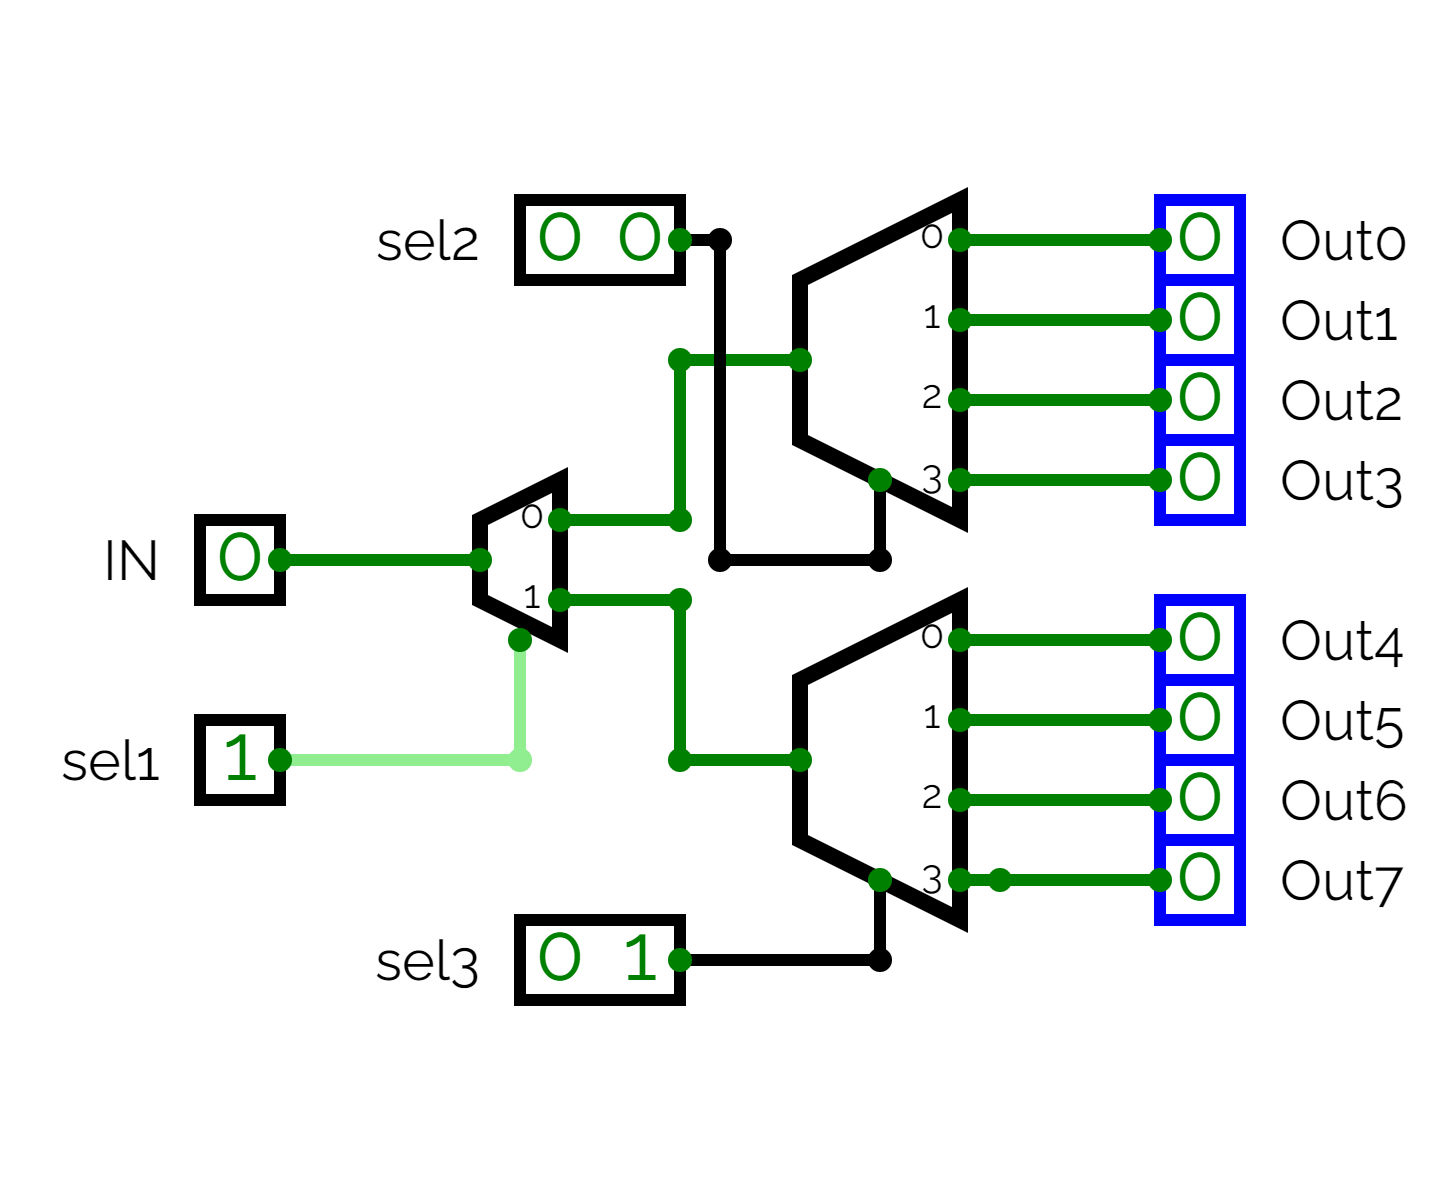
\includegraphics[width=1\textwidth]{CIRCUITOS/INT/Dmux8way_int.png}            \caption{Circuito interior de DMux8Way \cite{circuitverse}}
            \label{fig:dmux8way_int}
        \end{figure}
    \subsection{Esquema del circuito exterior}
        \begin{figure}[H]
            \centering
            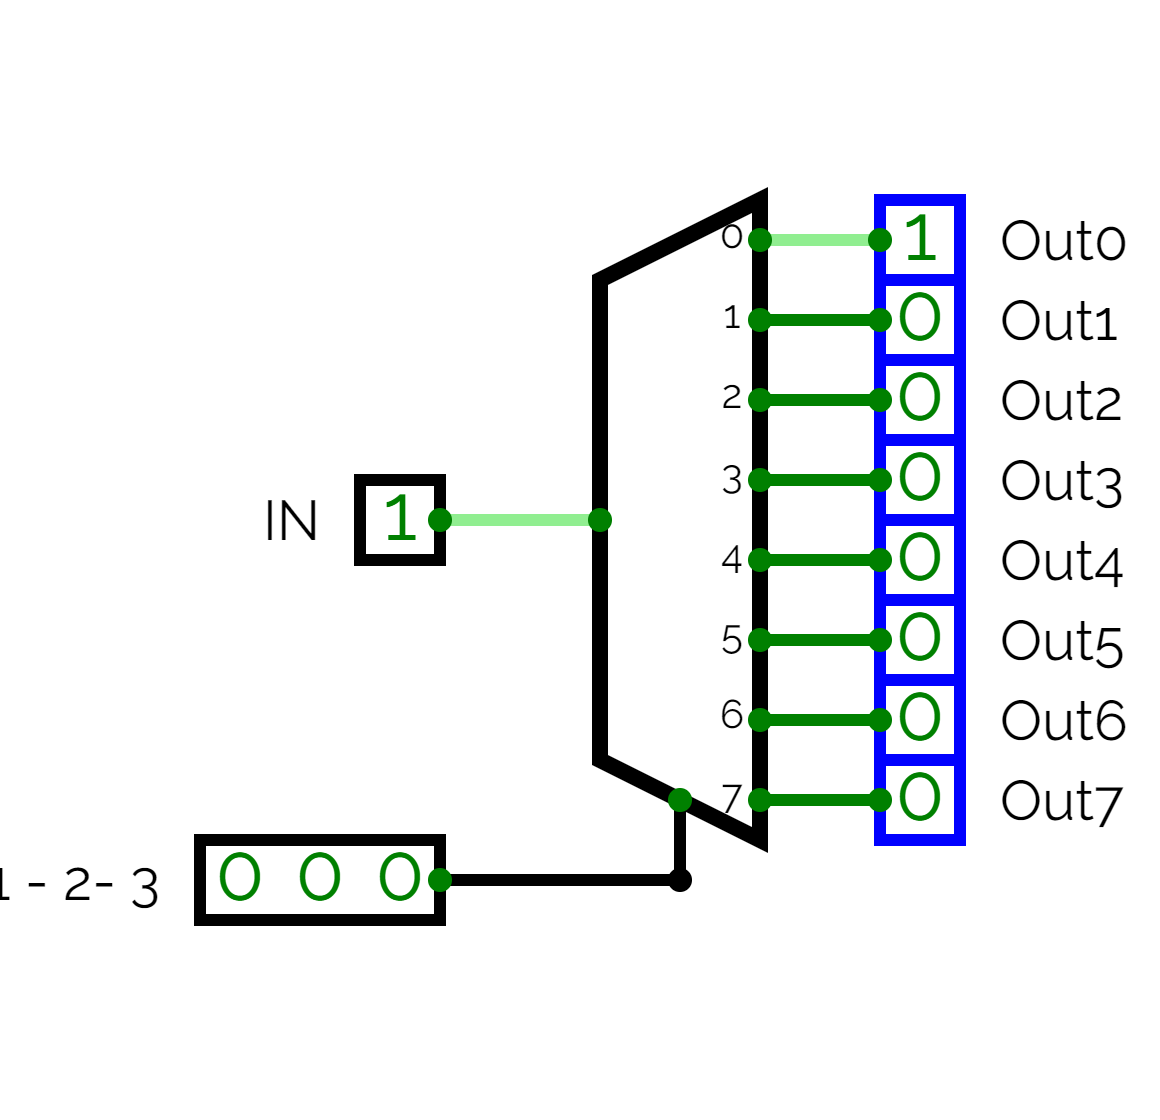
\includegraphics[width=1\textwidth]{CIRCUITOS/EXT/DMUX8WAY_ext.png}            \caption{Circuito exterior de DMux8Way \cite{circuitverse}}
            \label{fig:dmux8way_ext}
        \end{figure}
    \subsection{Implementación HDL}
        \begin{figure}[H]
            \centering
            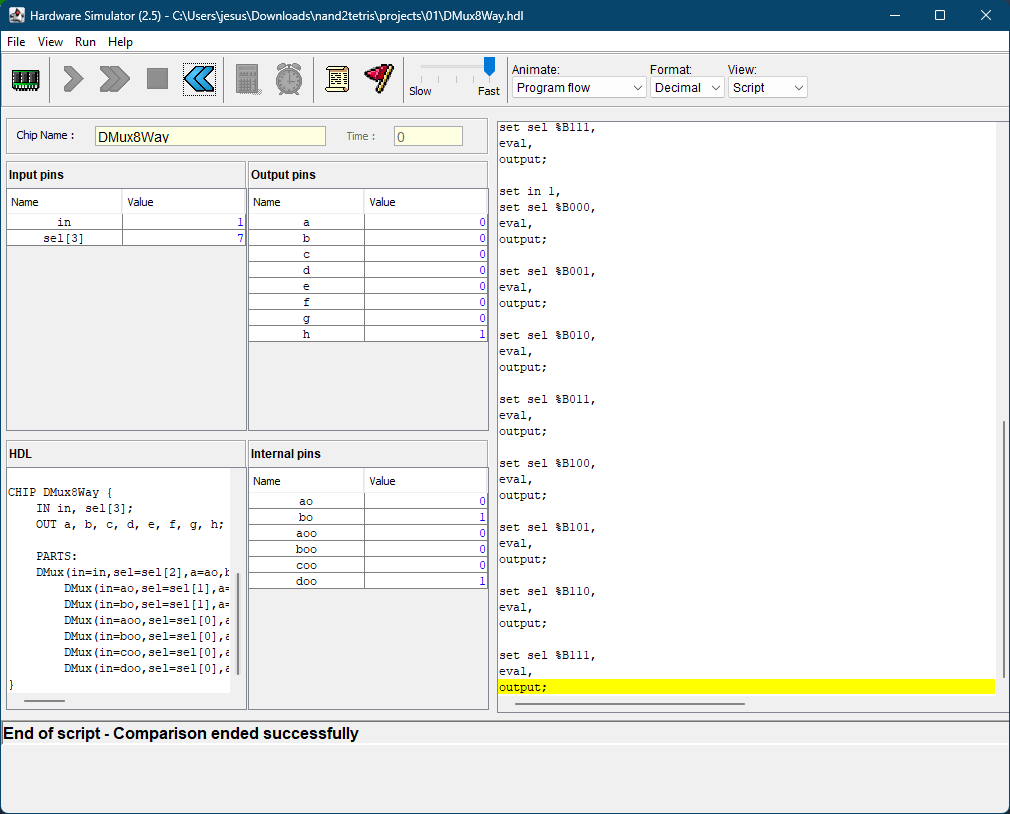
\includegraphics[width=0.75\linewidth]{CIRCUITOS//HDL/dmux8way.png}
            \caption{Test en Hardware Simulator de DMux8Way \cite{nand2tetris}}
            \label{fig:hdldmux8way}
        \end{figure}
        \subsubsection{Archivo HDL}
            \begin{lstlisting}
        CHIP DMux8Way {
            IN in, sel[3];
            OUT a, b, c, d, e, f, g, h;
        
            PARTS:
                DMux(in=in,sel=sel[2],a=ao,b=bo);
                DMux(in=ao,sel=sel[1],a=aoo,b=boo);
                DMux(in=bo,sel=sel[1],a=coo,b=doo);
                DMux(in=aoo,sel=sel[0],a=a,b=b);
                DMux(in=boo,sel=sel[0],a=c,b=d);
                DMux(in=coo,sel=sel[0],a=e,b=f);
                DMux(in=doo,sel=sel[0],a=g,b=h);
        }
            \end{lstlisting}
    \newpage

%%%%%%%%%%%%%%%%%%%%%%%%%%%%%%%%%%%%%%%%%%%%%%%%%%%%%%%%%%%%%%%%%%%%%%%%%%
%%%%%%%%%%%%%%%%%%%%%%%%%%%%%%%%%%%%%%%%%%%%%%%%%%%%%%%%%%%%%%%%%%%%%%%%%%

\section{Mux4Way16 (Muxi4o1b16)} \label{mux4waytitle}
    \subsection{Tabla de verdad y explicación del circuito}
        Un multiplexador de \textit{M}-vías y \textit{N}-bits selecciona un bit de un input y lo transfiere a un output de 1 bit. La selección se produce mediante una colección de control bits de número \textit{k}, con fórmula $k = log_{2}m$. \cite{nisan_nand2tetris_2005} \label{mux4way}
        \begin{table}[H]
        \centering
        \caption{Tabla de verdad de MUX4WAY16}
        \label{tab:tab_mux4way16}
        \resizebox{\textwidth}{!}{%
        \begin{tabular}{@{}llllll@{}}
        \toprule
        \texttt{a}                & \texttt{b}                & \texttt{c}                & \texttt{d}                & \texttt{sel} & \texttt{out}              \\ \midrule
        \texttt{0000000000000000} & \texttt{0000000000000000} & \texttt{0000000000000000} & \texttt{0000000000000000} & \texttt{00}  & \texttt{0000000000000000} \\
        \texttt{0000000000000000} & \texttt{0000000000000000} & \texttt{0000000000000000} & \texttt{0000000000000000} & \texttt{01}  & \texttt{0000000000000000} \\
        \texttt{0000000000000000} & \texttt{0000000000000000} & \texttt{0000000000000000} & \texttt{0000000000000000} & \texttt{10}  & \texttt{0000000000000000} \\ \midrule
        \texttt{0000000000000000} & \texttt{0000000000000000} & \texttt{0000000000000000} & \texttt{0000000000000000} & \texttt{11}  & \texttt{0000000000000000} \\
        \texttt{0001001000110100} & \texttt{1001100001110110} & \texttt{1010101010101010} & \texttt{0101010101010101} & \texttt{00}  & \texttt{0001001000110100} \\
        \texttt{0001001000110100} & \texttt{1001100001110110} & \texttt{1010101010101010} & \texttt{0101010101010101} & \texttt{01}  & \texttt{1001100001110110} \\
        \texttt{0001001000110100} & \texttt{1001100001110110} & \texttt{1010101010101010} & \texttt{0101010101010101} & \texttt{10}  & \texttt{1010101010101010} \\
        \texttt{0001001000110100} & \texttt{1001100001110110} & \texttt{1010101010101010} & \texttt{0101010101010101} & \texttt{11} & \textit{\texttt{0101010101010101}} \\ \bottomrule
        \end{tabular}%
        }
        \end{table}

    \subsection{Esquema del circuito interior}
        \begin{figure}[H]
            \centering
            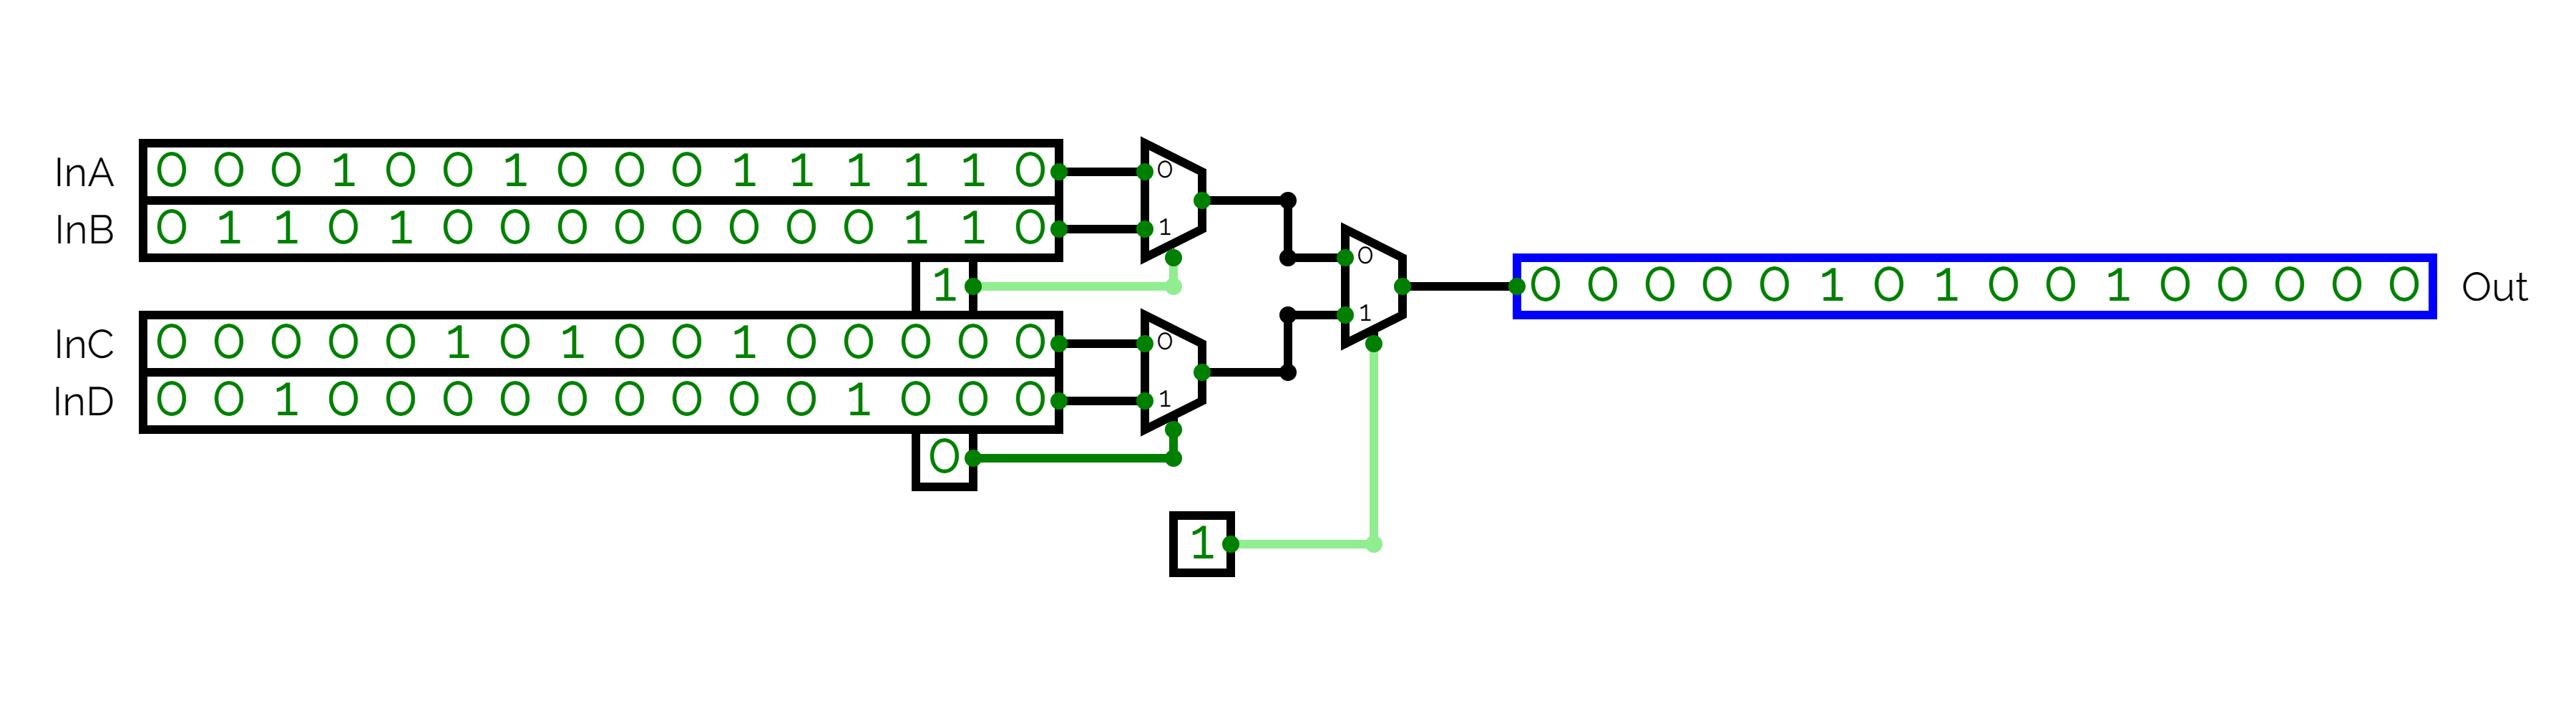
\includegraphics[width=1\textwidth]{CIRCUITOS/INT/Mux4Way16_int.png}            \caption{Circuito interior de Mux4Way16 \cite{circuitverse}}
            \label{fig:mux4way16_int}
        \end{figure}
    \subsection{Esquema del circuito exterior}
        \begin{figure}[H]
            \centering
            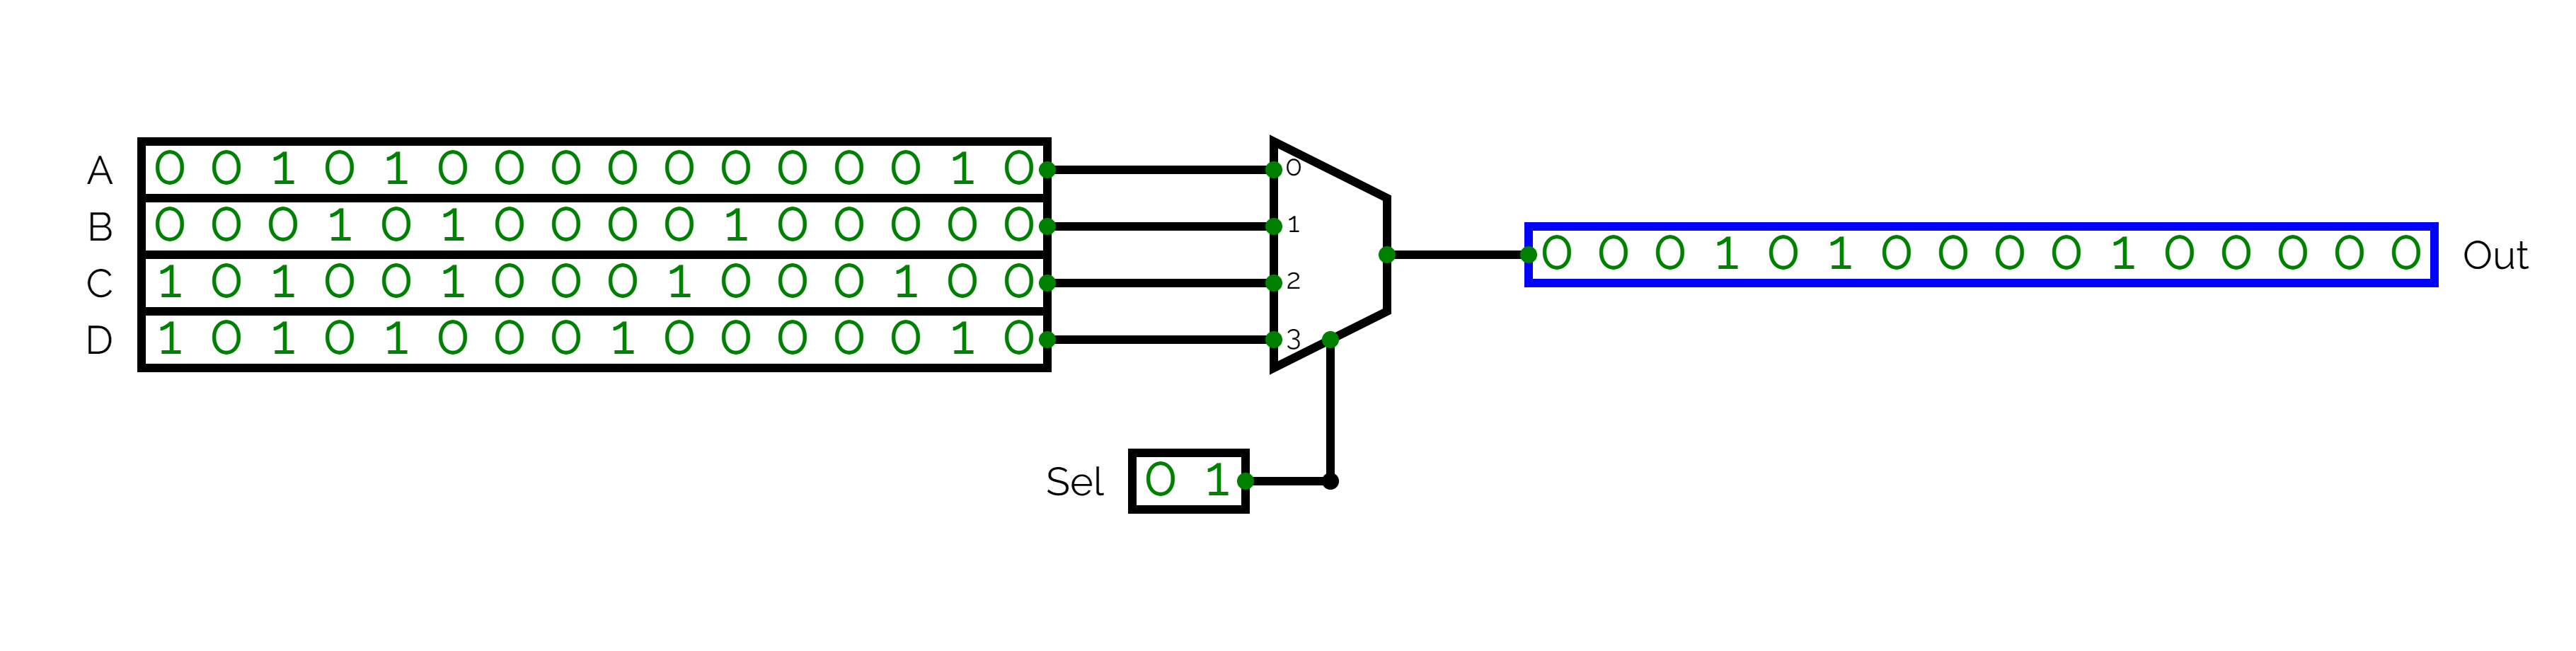
\includegraphics[width=1\textwidth]{CIRCUITOS/EXT/Mux4Way16_ext.png}            \caption{Circuito exterior de Mux4Way16 \cite{circuitverse}}
            \label{fig:mux4way16_ext}
        \end{figure}
    \subsection{Implementación HDL}
        \begin{figure}[H]
            \centering
            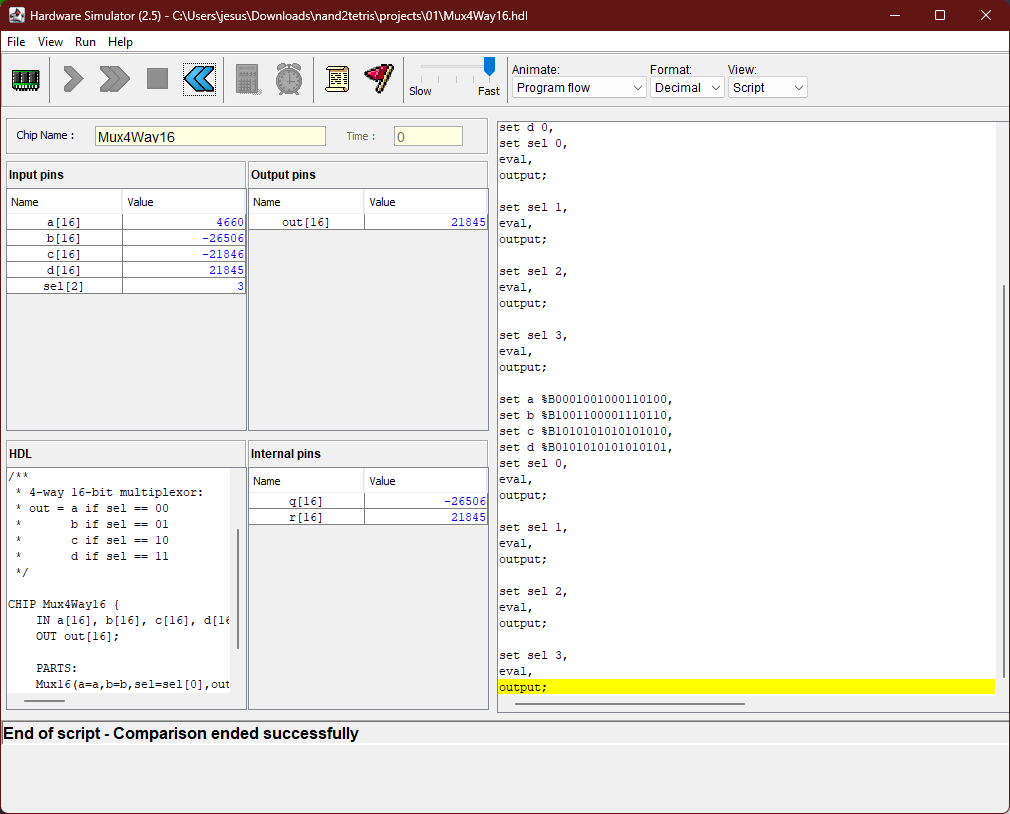
\includegraphics[width=0.75\linewidth]{mux4way16.png}
            \caption{Test en Hardware Simulator de Mux4Way16 \cite{nand2tetris}}
            \label{fig:hdlmux4way16}
        \end{figure}
        \subsubsection{Archivo HDL}
            \begin{lstlisting}
        CHIP Mux4Way16 {
            IN a[16], b[16], c[16], d[16], sel[2];
            OUT out[16];
        
            PARTS:
                Mux16(a=a,b=b,sel=sel[0],out=q); 
           	Mux16(a=c,b=d,sel=sel[0],out=r);
        	Mux16(a=q,b=r,sel=sel[1],out=out);
        }
            \end{lstlisting}
    \newpage

%%%%%%%%%%%%%%%%%%%%%%%%%%%%%%%%%%%%%%%%%%%%%%%%%%%%%%%%%%%%%%%%%%%%%%%%%%
%%%%%%%%%%%%%%%%%%%%%%%%%%%%%%%%%%%%%%%%%%%%%%%%%%%%%%%%%%%%%%%%%%%%%%%%%%

\section{Mux8Way16 (Muxi8o1b16)}
    \subsection{Tabla de verdad y explicación del circuito}
        Mismo circuito que se ha visto en: \ref{mux4waytitle}, con la descripción: \ref{mux4way}. En pocas palabras, es un multiplexador de 8 puertas, en lugar de 4. \cite{nisan_nand2tetris_2005}
        \begin{table}[H]
        \centering
        \caption{Tabla de verdad de MUX8WAY16}
        \label{tab:tab_mux8way16}
        \resizebox{\columnwidth}{!}{%
        \begin{tabular}{@{}llllllllll@{}}
        \toprule
        \multicolumn{1}{c}{\texttt{a}} &
          \multicolumn{1}{c}{\texttt{b}} &
          \multicolumn{1}{c}{\texttt{c}} &
          \multicolumn{1}{c}{\texttt{d}} &
          \multicolumn{1}{c}{\texttt{e}} &
          \multicolumn{1}{c}{\texttt{f}} &
          \multicolumn{1}{c}{\texttt{g}} &
          \multicolumn{1}{c}{\texttt{h}} &
          \multicolumn{1}{c}{\texttt{sel}} &
          \multicolumn{1}{c}{\texttt{out}} \\ \midrule
        \texttt{0000000000000000} &
          \texttt{0000000000000000} &
          \texttt{0000000000000000} &
          \texttt{0000000000000000} &
          \texttt{0000000000000000} &
          \texttt{0000000000000000} &
          \texttt{0000000000000000} &
          \texttt{0000000000000000} &
          \texttt{000} &
          \texttt{0000000000000000} \\
        \texttt{0000000000000000} &
          \texttt{0000000000000000} &
          \texttt{0000000000000000} &
          \texttt{0000000000000000} &
          \texttt{0000000000000000} &
          \texttt{0000000000000000} &
          \texttt{0000000000000000} &
          \texttt{0000000000000000} &
          \texttt{001} &
          \texttt{0000000000000000} \\
        \texttt{0000000000000000} &
          \texttt{0000000000000000} &
          \texttt{0000000000000000} &
          \texttt{0000000000000000} &
          \texttt{0000000000000000} &
          \texttt{0000000000000000} &
          \texttt{0000000000000000} &
          \texttt{0000000000000000} &
          \texttt{010} &
          \texttt{0000000000000000} \\
        \texttt{0000000000000000} &
          \texttt{0000000000000000} &
          \texttt{0000000000000000} &
          \texttt{0000000000000000} &
          \texttt{0000000000000000} &
          \texttt{0000000000000000} &
          \texttt{0000000000000000} &
          \texttt{0000000000000000} &
          \texttt{011} &
          \texttt{0000000000000000} \\
        \texttt{0000000000000000} &
          \texttt{0000000000000000} &
          \texttt{0000000000000000} &
          \texttt{0000000000000000} &
          \texttt{0000000000000000} &
          \texttt{0000000000000000} &
          \texttt{0000000000000000} &
          \texttt{0000000000000000} &
          \texttt{100} &
          \texttt{0000000000000000} \\
        \texttt{0000000000000000} &
          \texttt{0000000000000000} &
          \texttt{0000000000000000} &
          \texttt{0000000000000000} &
          \texttt{0000000000000000} &
          \texttt{0000000000000000} &
          \texttt{0000000000000000} &
          \texttt{0000000000000000} &
          \texttt{101} &
          \texttt{0000000000000000} \\
        \texttt{0000000000000000} &
          \texttt{0000000000000000} &
          \texttt{0000000000000000} &
          \texttt{0000000000000000} &
          \texttt{0000000000000000} &
          \texttt{0000000000000000} &
          \texttt{0000000000000000} &
          \texttt{0000000000000000} &
          \texttt{110} &
          \texttt{0000000000000000} \\
        \texttt{0000000000000000} &
          \texttt{0000000000000000} &
          \texttt{0000000000000000} &
          \texttt{0000000000000000} &
          \texttt{0000000000000000} &
          \texttt{0000000000000000} &
          \texttt{0000000000000000} &
          \texttt{0000000000000000} &
          \texttt{111} &
          \texttt{0000000000000000} \\
        \texttt{0001001000110100} &
          \texttt{0010001101000101} &
          \texttt{0011010001010110} &
          \texttt{0100010101100111} &
          \texttt{0101011001111000} &
          \texttt{0110011110001001} &
          \texttt{0111100010011010} &
          \texttt{1000100110101011} &
          \texttt{000} &
          \texttt{0001001000110100} \\
        \texttt{0001001000110100} &
          \texttt{0010001101000101} &
          \texttt{0011010001010110} &
          \texttt{0100010101100111} &
          \texttt{0101011001111000} &
          \texttt{0110011110001001} &
          \texttt{0111100010011010} &
          \texttt{1000100110101011} &
          \texttt{001} &
          \texttt{0010001101000101} \\
        \texttt{0001001000110100} &
          \texttt{0010001101000101} &
          \texttt{0011010001010110} &
          \texttt{0100010101100111} &
          \texttt{0101011001111000} &
          \texttt{0110011110001001} &
          \texttt{0111100010011010} &
          \texttt{1000100110101011} &
          \texttt{010} &
          \texttt{0011010001010110} \\
        \texttt{0001001000110100} &
          \texttt{0010001101000101} &
          \texttt{0011010001010110} &
          \texttt{0100010101100111} &
          \texttt{0101011001111000} &
          \texttt{0110011110001001} &
          \texttt{0111100010011010} &
          \texttt{1000100110101011} &
          \texttt{011} &
          \texttt{0100010101100111} \\
        \texttt{0001001000110100} &
          \texttt{0010001101000101} &
          \texttt{0011010001010110} &
          \texttt{0100010101100111} &
          \texttt{0101011001111000} &
          \texttt{0110011110001001} &
          \texttt{0111100010011010} &
          \texttt{1000100110101011} &
          \texttt{100} &
          \texttt{0101011001111000} \\
        \texttt{0001001000110100} &
          \texttt{0010001101000101} &
          \texttt{0011010001010110} &
          \texttt{0100010101100111} &
          \texttt{0101011001111000} &
          \texttt{0110011110001001} &
          \texttt{0111100010011010} &
          \texttt{1000100110101011} &
          \texttt{101} &
          \texttt{0110011110001001} \\
        \texttt{0001001000110100} &
          \texttt{0010001101000101} &
          \texttt{0011010001010110} &
          \texttt{0100010101100111} &
          \texttt{0101011001111000} &
          \texttt{0110011110001001} &
          \texttt{0111100010011010} &
          \texttt{1000100110101011} &
          \texttt{110} &
          \texttt{0111100010011010} \\
        \texttt{0001001000110100} &
          \texttt{0010001101000101} &
          \texttt{0011010001010110} &
          \texttt{0100010101100111} &
          \texttt{0101011001111000} &
          \texttt{0110011110001001} &
          \texttt{0111100010011010} &
          \texttt{1000100110101011} &
          \texttt{111} &
          \texttt{1000100110101011} \\ \bottomrule
        \end{tabular}%
        }
        \end{table}

    \subsection{Esquema del circuito interior}
        \begin{figure}[H]
            \centering
            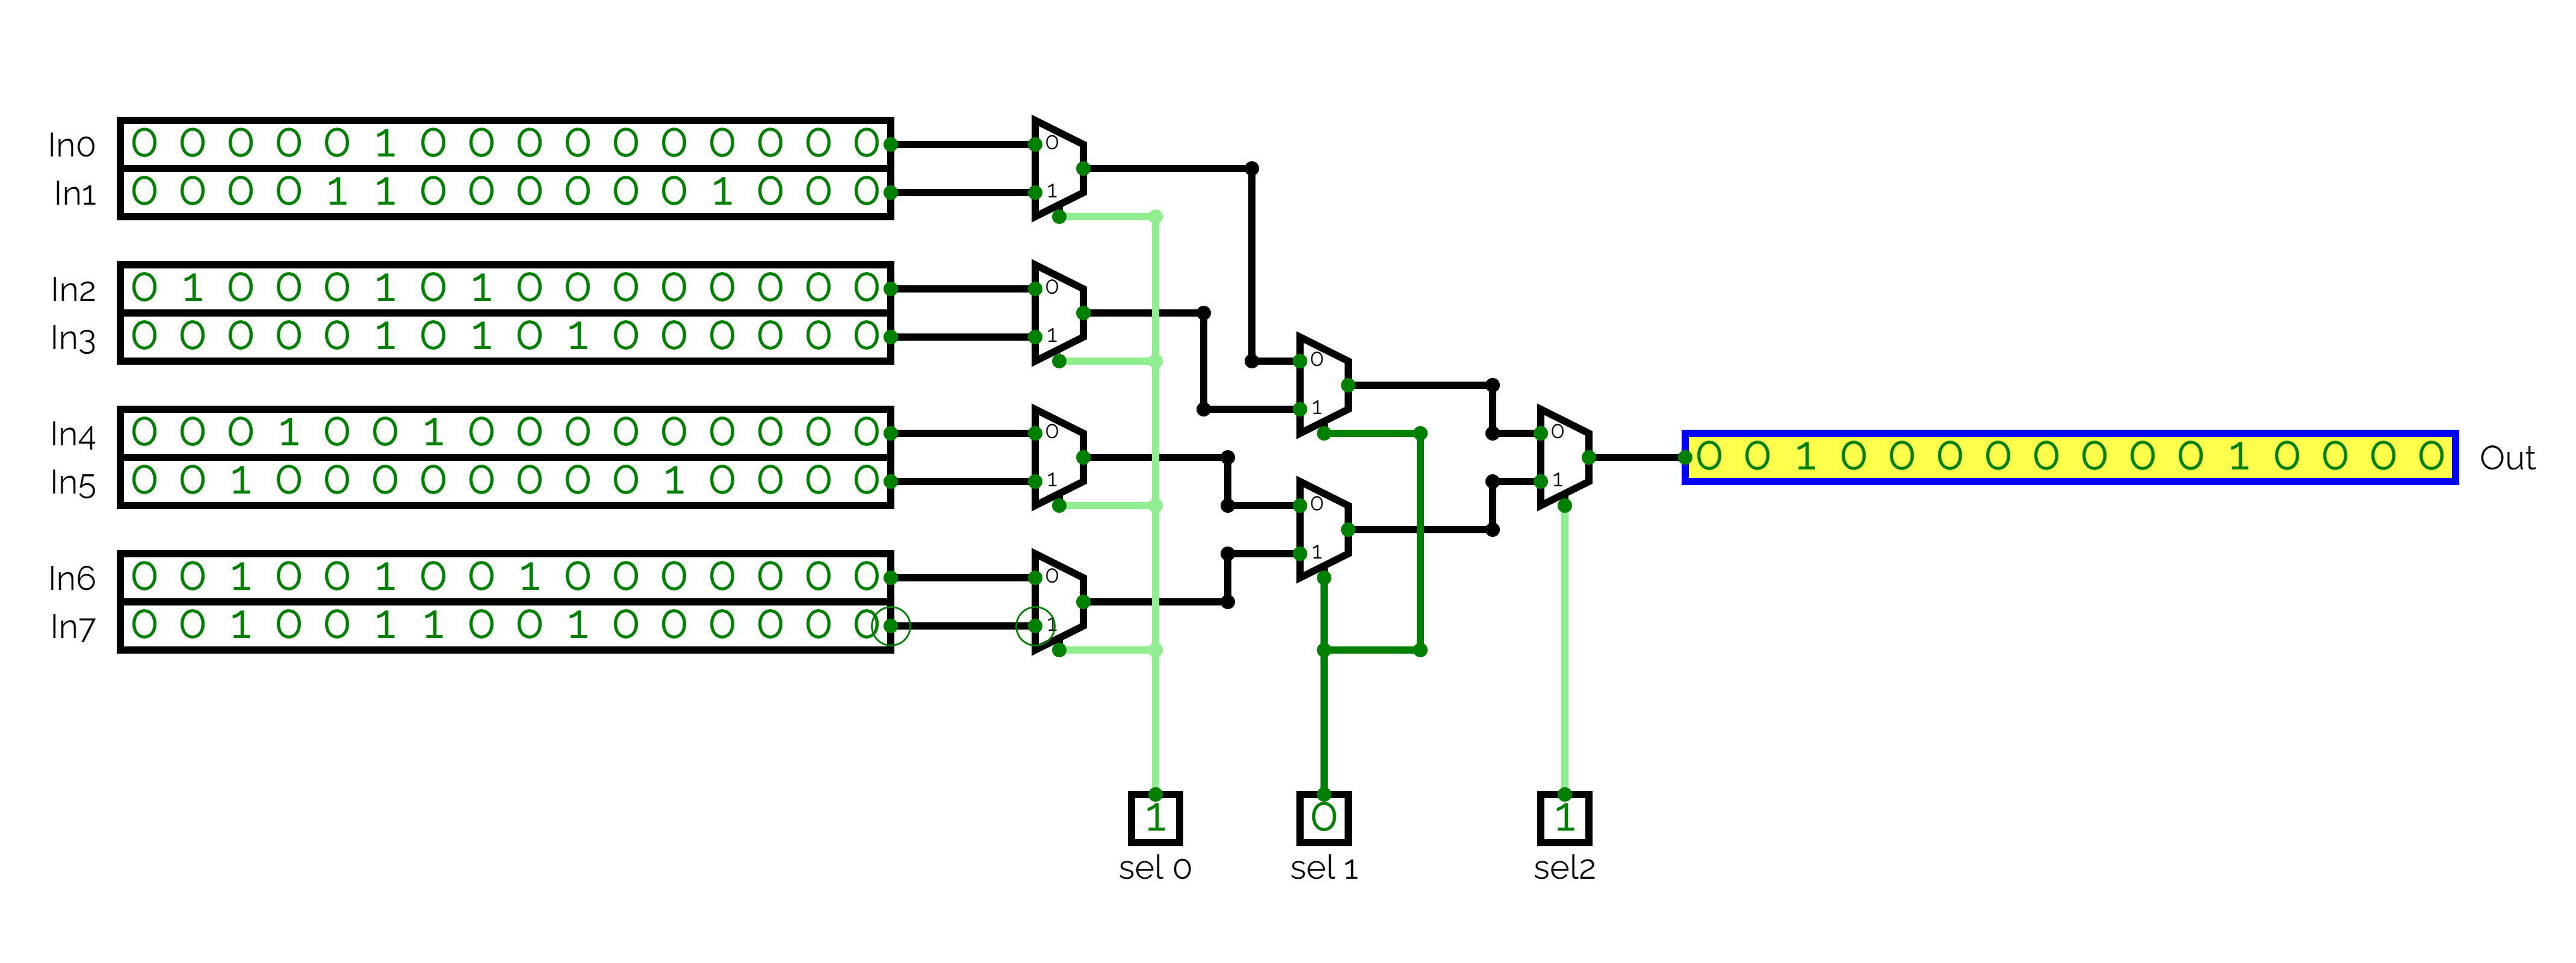
\includegraphics[width=1\textwidth]{CIRCUITOS/INT/Mux8Way16_int.png}            \caption{Circuito interior de Mux8Way16 \cite{circuitverse}}
            \label{fig:mux8way16_int}
        \end{figure}
    \subsection{Esquema del circuito exterior}
        \begin{figure}[H]
            \centering
            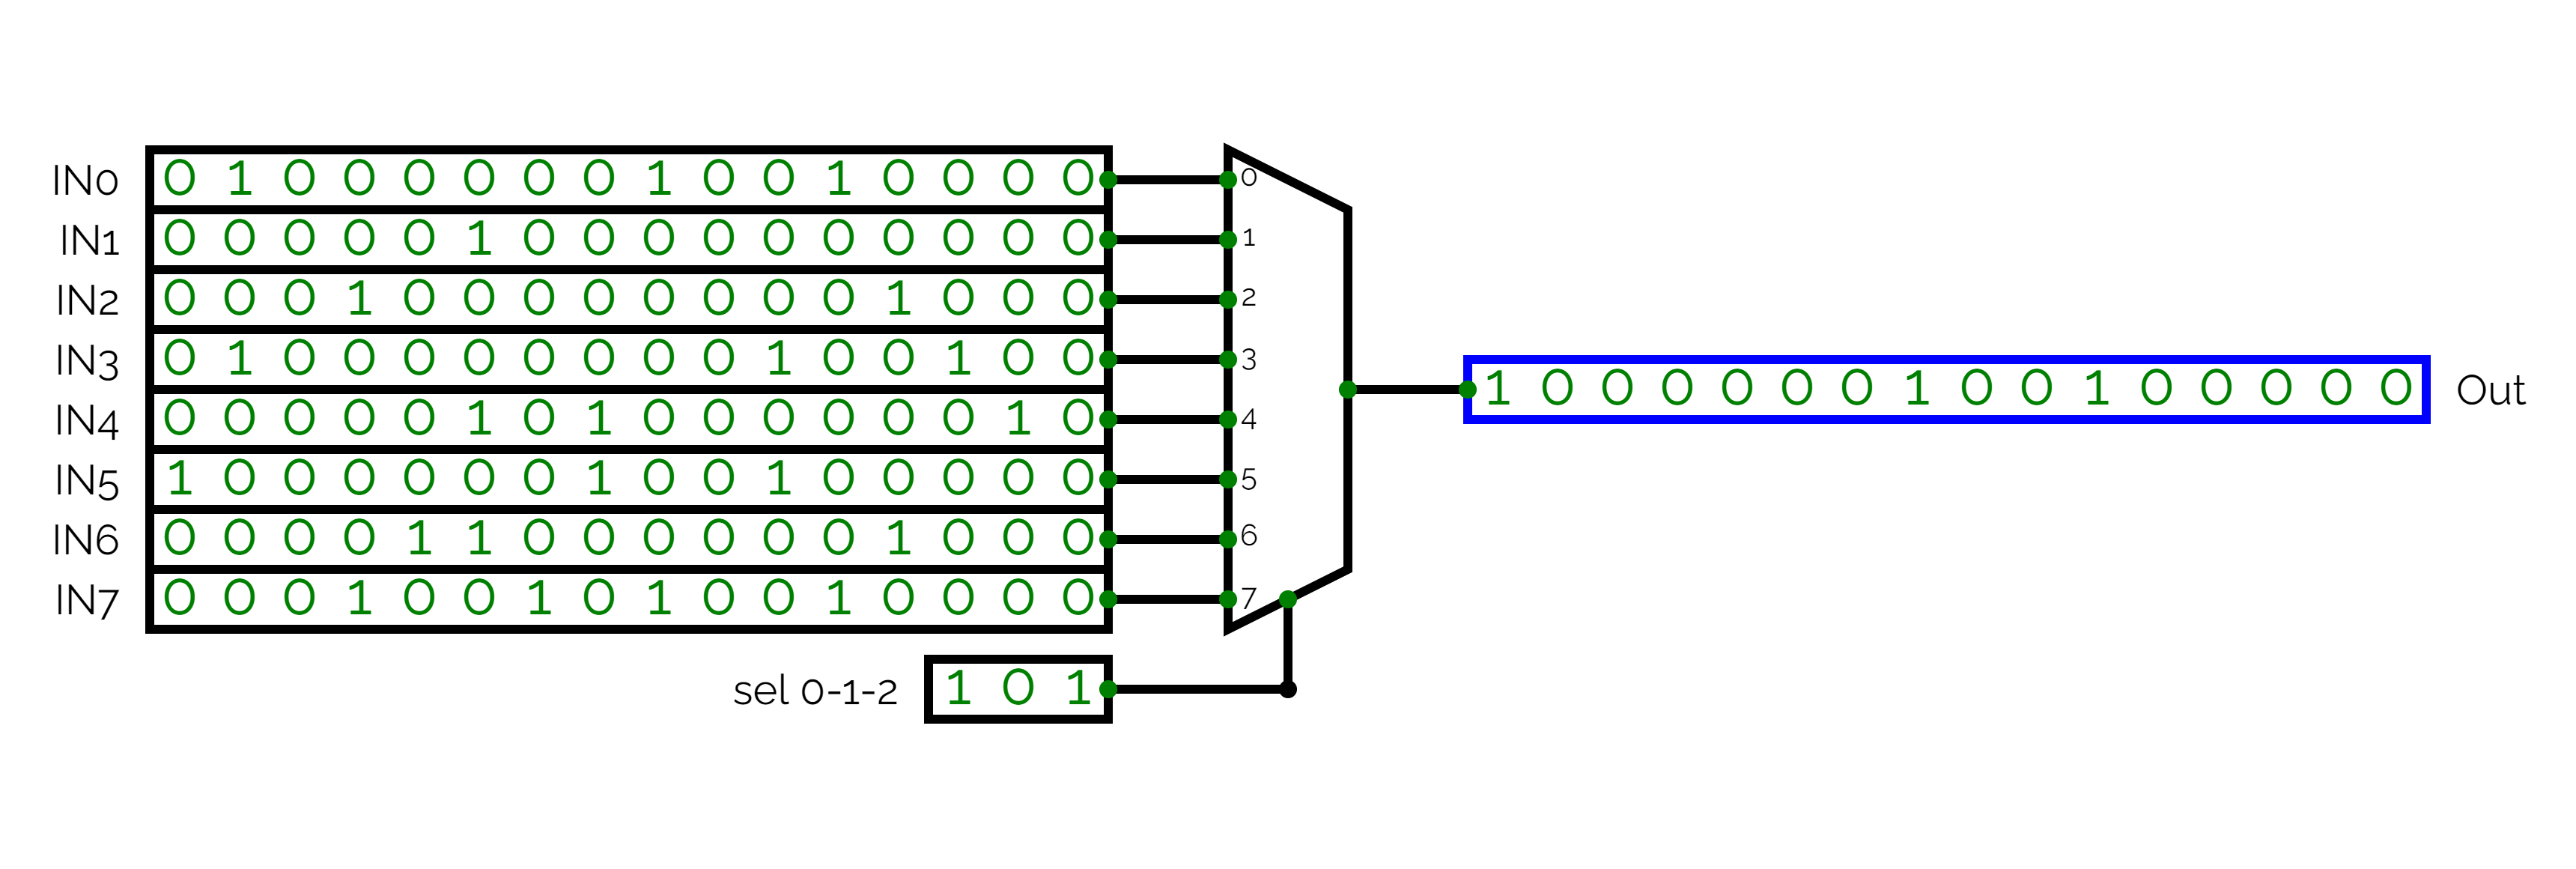
\includegraphics[width=1\textwidth]{CIRCUITOS/EXT/MUX8WAY16_ext.png}            
            \caption{Circuito exterior de Mux8Way16 \cite{circuitverse}}
            \label{fig:mux8way16_ext}
        \end{figure}
    \subsection{Implementación HDL}
        \begin{figure}[H]
            \centering
            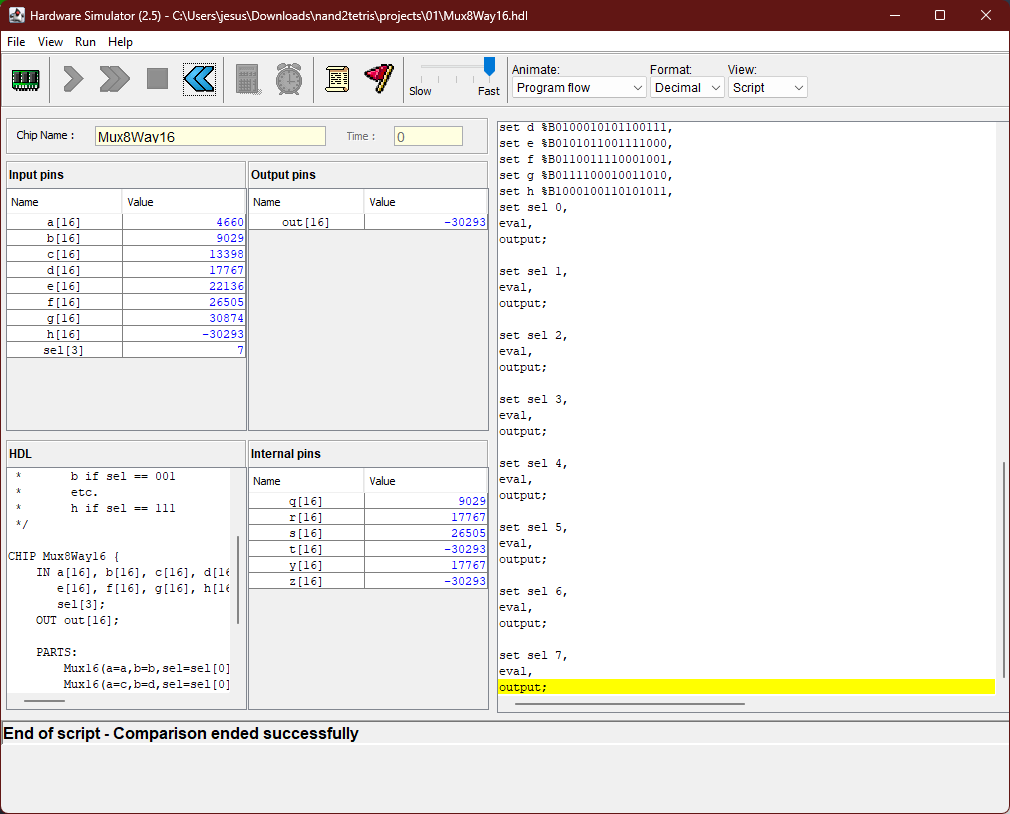
\includegraphics[width=0.75\linewidth]{CIRCUITOS//HDL/mux8way16_hdl.png}
            \caption{Test en Hardware Simulator de Mux8Way16 \cite{nand2tetris}}
            \label{fig:hdlmux8way16}
        \end{figure}
        \subsubsection{Archivo HDL}
            \begin{lstlisting}
        CHIP Mux8Way16 {
        IN a[16], b[16], c[16], d[16],
           e[16], f[16], g[16], h[16],
           sel[3];
        OUT out[16];
    
        PARTS:
            Mux16(a=a,b=b,sel=sel[0],out=q); 
            Mux16(a=c,b=d,sel=sel[0],out=r);
            Mux16(a=e,b=f,sel=sel[0],out=s); 
            Mux16(a=g,b=h,sel=sel[0],out=t);
            Mux16(a=q,b=r,sel=sel[1],out=y);
            Mux16(a=s,b=t,sel=sel[1],out=z);
            Mux16(a=y,b=z,sel=sel[2],out=out);
        }
            \end{lstlisting}
    \newpage


%%%%%%%%%%%%%%%%%%%%%%%%%%%%%%%%%%%%%%%%%%%%%%%%%%%%%%%%%%%%%%%%%%%%%%%%%%
%%%%%%%%%%%%%%%%%%%%%%%%%%%%%%%%%%%%%%%%%%%%%%%%%%%%%%%%%%%%%%%%%%%%%%%%%%

\section{Or8Way (Ori8o1b1)}
    \subsection{Tabla de verdad y explicación del circuito}
        Un Or de \textit{N}-puertas produce en el output un 1 cuando \textit{al menos} uno de los inputs es 1, y 0 en caso contrario. \cite{nisan_nand2tetris_2005}
        \begin{table}[H]
        \centering
        \caption{Tabla de verdad de Or8Way}
        \label{tab:tab_Or8way}
        \resizebox{0.25\textwidth}{!}{%
        \begin{tabular}{@{}ll@{}}
        \toprule
        \texttt{in}       & \texttt{out} \\ \midrule
        \texttt{00000000} & \texttt{0}   \\
        \texttt{11111111} & \texttt{1}   \\
        \texttt{00010000} & \texttt{1}   \\
        \texttt{00000001} & \texttt{1}   \\
        \texttt{00100110} & \texttt{1}   \\ \bottomrule
        \end{tabular}%
        }
        \end{table}
        
    \subsection{Esquema del circuito interior}
        \begin{figure}[H]
            \centering
            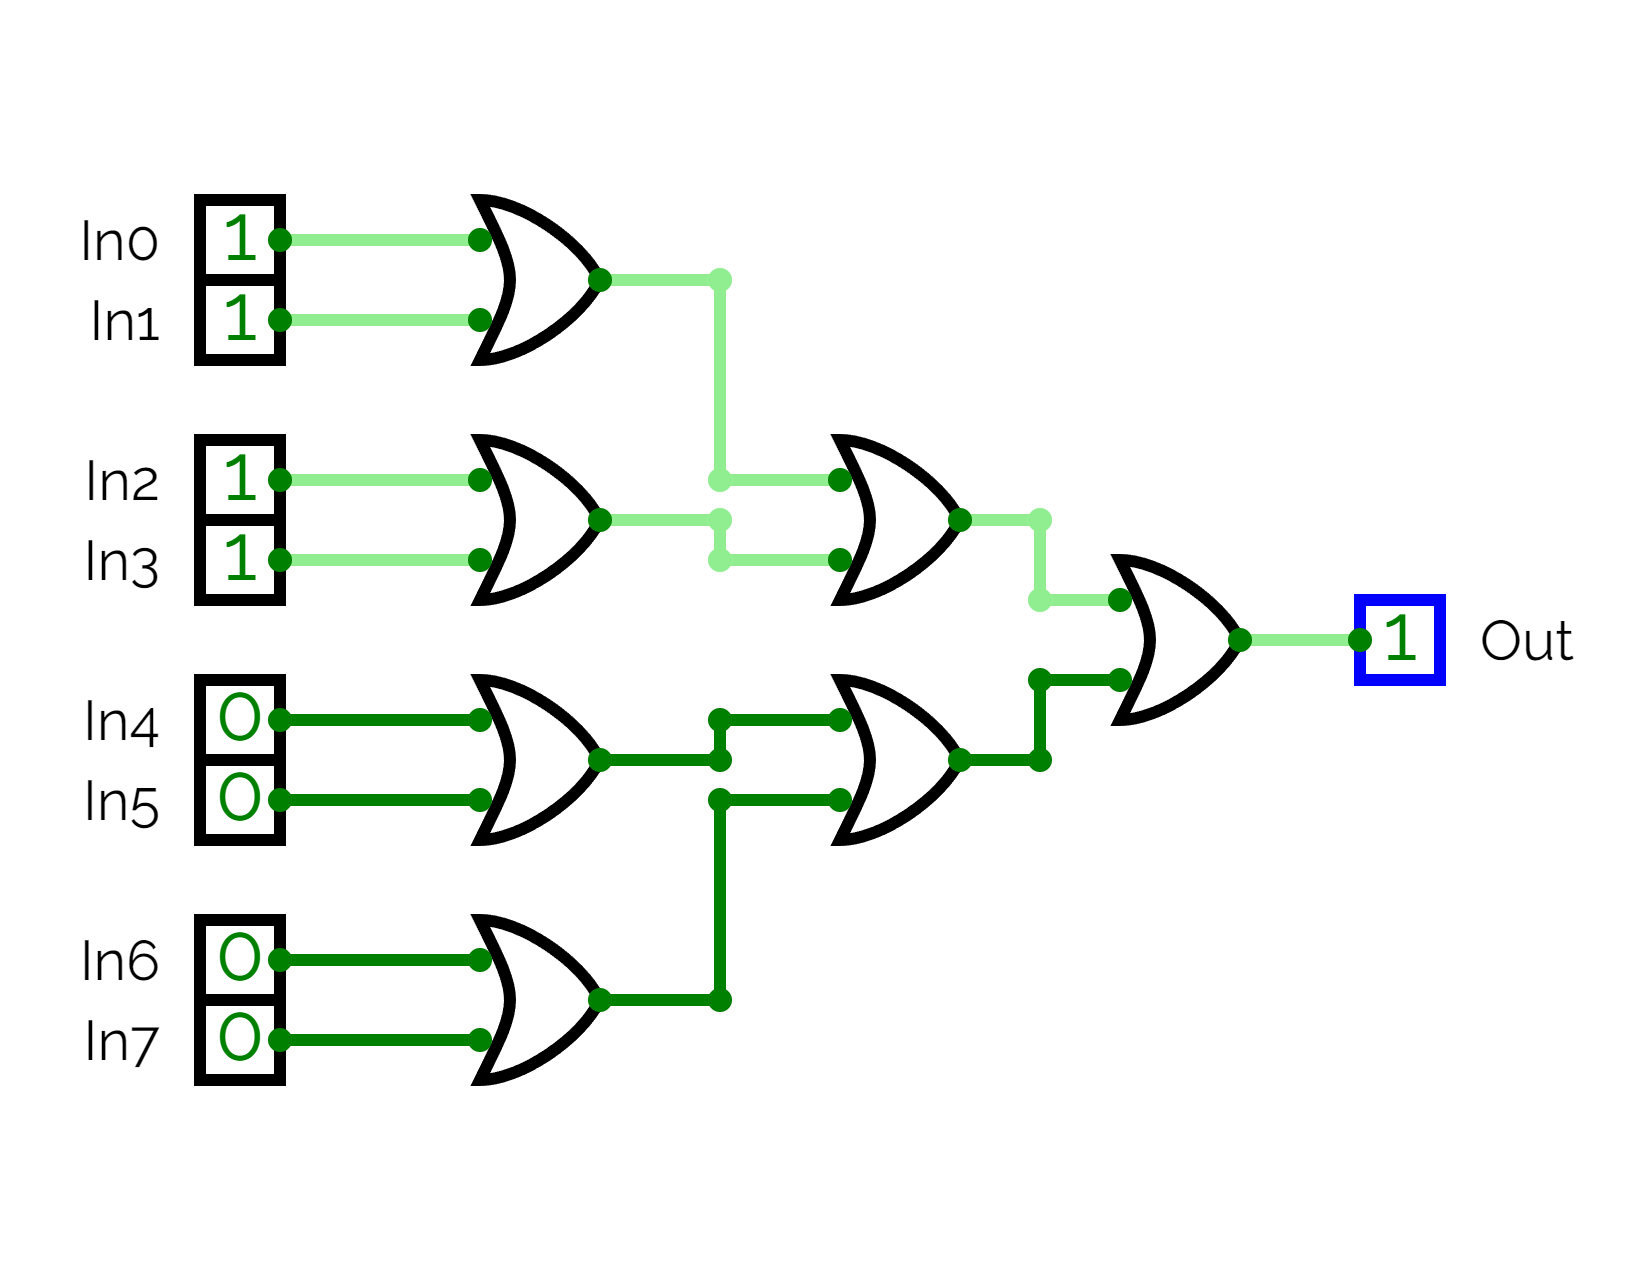
\includegraphics[width=1\textwidth]{CIRCUITOS/INT/OR8Way_int.png}            \caption{Circuito interior de Or8Way \cite{circuitverse}}
            \label{fig:or8way_int}
        \end{figure}
    \subsection{Esquema del circuito exterior}
        \begin{figure}[H]
            \centering
            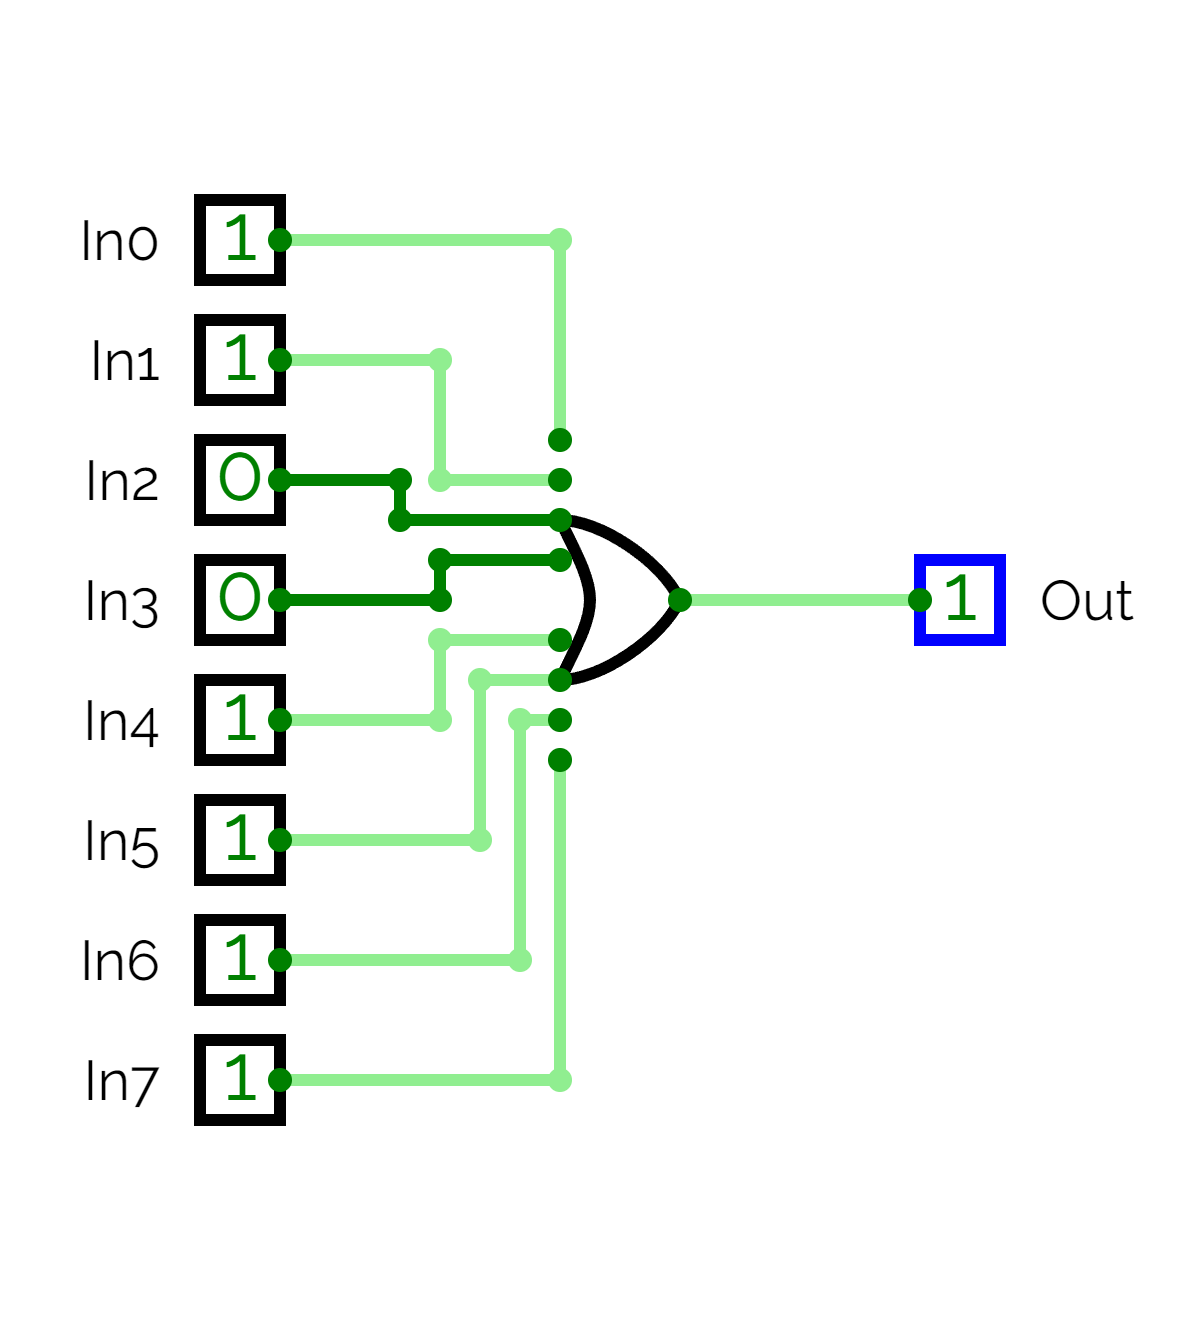
\includegraphics[width=0.8\textwidth]{CIRCUITOS/EXT/Or8Way_ext.png}            \caption{Circuito exterior de Or8Way \cite{circuitverse}}
            \label{fig:or8way_ext}
        \end{figure}
    \subsection{Implementación HDL}
        \begin{figure}[H]
            \centering
            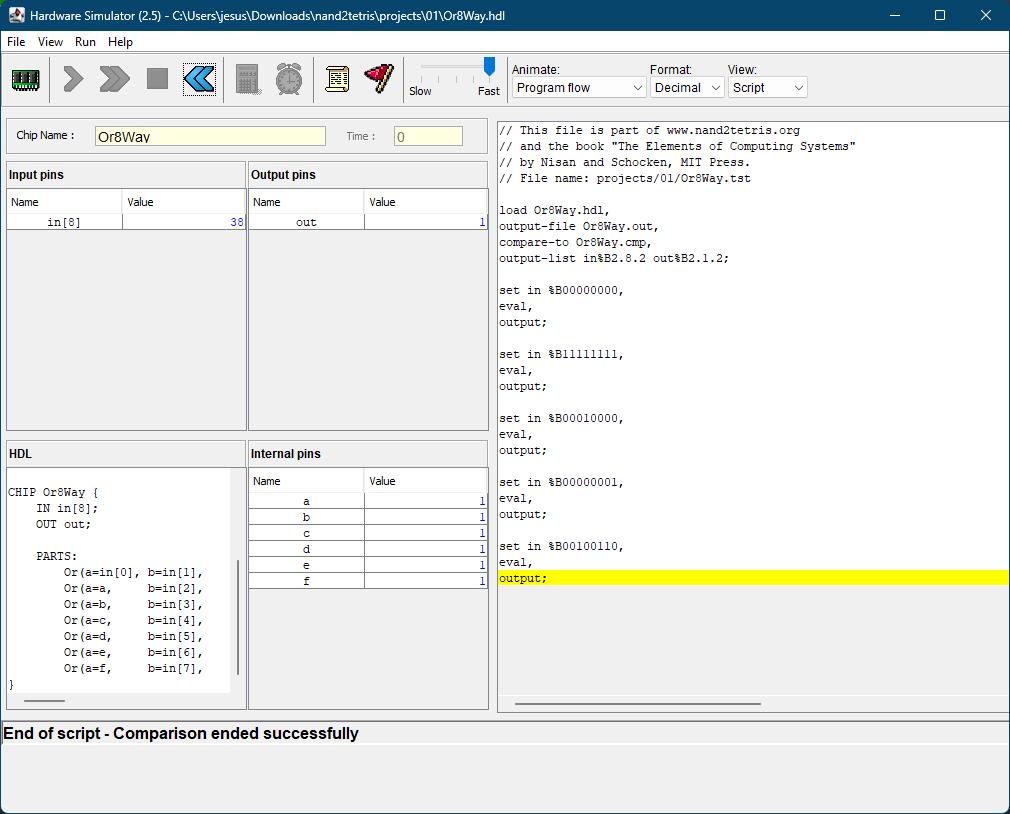
\includegraphics[width=0.75\linewidth]{CIRCUITOS//HDL/or8way.png}
            \caption{Test en Hardware Simulator de Or8Way \cite{nand2tetris}}
            \label{fig:hdlor8way}
        \end{figure}
        \subsubsection{Archivo HDL}
            \begin{lstlisting}
        CHIP Or8Way {
            IN in[8];
            OUT out;
        
            PARTS:
                Or(a=in[0], b=in[1],     out=a);
                Or(a=a,     b=in[2],     out=b);
                Or(a=b,     b=in[3],     out=c);
                Or(a=c,     b=in[4],     out=d);
                Or(a=d,     b=in[5],     out=e);
                Or(a=e,     b=in[6],     out=f);
                Or(a=f,     b=in[7],     out=out);
        }
            \end{lstlisting}
    \newpage
\newpage

\printbibliography[heading=bibintoc]
\end{document}
